\documentclass[pldi]{sigplanconf}

%% =============================================================
\def\tool{\textsc{Tool}\xspace}
\def\papertitle{\tool: Program Repairing using Exception Types, Constraint
Automata and Typestate}
\def\pdfauthors{}
\def\paperkeywords{}
%% =============================================================

\usepackage{color}

\newcommand{\subparagraph}{}

% You can tweak clickable link colors here:
\definecolor{linkcol}{rgb}{0,0,1}
\definecolor{citecol}{rgb}{0,0.5,0}
\definecolor{urlcol}{rgb}{0.3,0,0}

% Make pdflatex use letter size --md
\setlength{\pdfpagewidth}{8.5in}
\setlength{\pdfpageheight}{11in}

\let\proof\relax
\let\endproof\relax

\usepackage{cite}
\usepackage{amsthm}
% \usepackage{amsmath}
% \usepackage{amsfonts}
\usepackage{ragged2e}
\usepackage{txfonts}
\usepackage{fancyhdr}
\usepackage{amssymb}
\usepackage{fancyvrb}
\usepackage{graphicx}
\usepackage{times}
\usepackage{pifont}
\usepackage[hyphens]{url}
\usepackage{xspace}
\usepackage{sty/algorithm2e}
%%\usepackage[belowskip=-10pt,aboveskip=5pt,small,labelfont=bf]{caption}
\usepackage[aboveskip=5pt,small,labelfont=bf]{caption}
\DeclareCaptionType{copyrightbox}
\usepackage[bookmarks=true,%
bookmarksnumbered=true,%
colorlinks=true,%
linkcolor=linkcol,%
citecolor=citecol,%
urlcolor=urlcol,%
hypertexnames=true,%
pdfpagelabels,
% draft
]{hyperref}

\hypersetup{%
  colorlinks=false,% hyperlinks will be black
  pdfborderstyle={/S/U/W 1}% border style will be underline of width 1pt
}

\usepackage{sty/multirow}
\usepackage{sty/flushend}
\usepackage{epstopdf}
\usepackage[small,compact]{sty/titlesec}
\usepackage[font=scriptsize]{subfig}
\usepackage{sty/wrapfig}

\usepackage{epstopdf}
\usepackage{fancybox}
\usepackage{listings}
\usepackage{xcolor}
%\usepackage[]{datetime}
%\usepackage{lipsum}

\newcommand{\ignore}[1]{}
% \usepackage{rotating}

%==========================================
%Added definitions
% \usepackage{amsthm}
\theoremstyle{definition}
\newtheorem{definition}{Definition}[section]
%==========================================
%rename listing
\renewcommand\lstlistingname{Code}
%==========================================

%==========================================
%rotate column title
\usepackage{booktabs}
% \usepackage{xparse}
% \NewDocumentCommand{\rot}{O{45} O{1em} m}{\makebox[#2][l]{\rotatebox{#1}{#3}}}
%==========================================

%==========================================
%Automatic row number in table
% \usepackage{array,etoolbox}
% \preto\tabular{\setcounter{magicrownumbers}{0}}
% \newcounter{magicrownumbers}
% \newcommand\rownumber{\stepcounter{magicrownumbers}\arabic{magicrownumbers}}
%==========================================
\SetAlFnt{\small}
\SetAlCapFnt{\small}
\SetAlCapNameFnt{\small}
\SetVlineSkip{0pt}

\setlength\floatsep{5pt}
\setlength\textfloatsep{5pt}
\setlength\intextsep{5pt}

\hypersetup{
pdfauthor = {},
pdftitle = {\papertitle},
pdfkeywords = {\paperkeywords},
pdfcreator = {LaTeX with hyperref package},
pdfproducer = {pdflatex}}

\definecolor{dkgreen}{rgb}{0,0.6,0}
\definecolor{gray}{rgb}{0.5,0.5,0.5}
\definecolor{mauve}{rgb}{0.58,0,0.82}

\lstset{%frame=tb,
  captionpos=b,
  language=Java,
  aboveskip=10pt,
  belowskip=0pt,
  abovecaptionskip=5pt,
  belowcaptionskip=5pt,
  numberblanklines=false,
  showstringspaces=false,
  columns=flexible,
  basicstyle={\scriptsize\ttfamily},
  numbers= left,
  numbersep=5pt,
  numberstyle=\scriptsize,
  %frame=single,
  numberstyle=\tiny\color{gray},
  keywordstyle=\color{blue},
  commentstyle=\color{dkgreen},
  stringstyle=\color{mauve},
  breaklines=true,
  breakatwhitespace=true
  tabsize=2,
  xleftmargin=2em,
  morecomment=[l]{//},
  escapeinside={<@}{@>},
}

\makeatletter
\lst@Key{countblanklines}{true}[t]%
    {\lstKV@SetIf{#1}\lst@ifcountblanklines}

\lst@AddToHook{OnEmptyLine}{%
    \lst@ifnumberblanklines\else%
       \lst@ifcountblanklines\else%
         \advance\c@lstnumber-\@ne\relax%
       \fi%
    \fi}
\makeatother

% Use a smaller font size for URLs:
\makeatletter
\def\url@myurlstyle{%
   \@ifundefined{selectfont}{\def\UrlFont{\small}}{\def\UrlFont{\small}}}
   \makeatother
\urlstyle{myurl}

% This adds ':' to the characters after which not to break URLs, and
% defines a smaller typewriter font. --cpk
% changed small to sf -- md
\def\UrlNoBreaks{\do:\do\(\do\[\do\{\do\<}%
\def\UrlFont{\small\ttfamily}
\def\UrlOrds{\do\*\do\~}%

% For referencing sections, Vern-style
\newcommand\xref[1]{\S~\ref{#1}}

% Black filled circles with white number on it
% See Comprehensive LaTeX Symbol List --cpk
\def\blackI{\ding{182}}
\def\blackII{\ding{183}}
\def\blackIII{\ding{184}}
\def\blackIV{\ding{185}}
\def\blackV{\ding{186}}
\def\blackVI{\ding{187}}

\def\first{({\it i})\xspace }
\def\second{({\it ii})\xspace }
\def\third{({\it iii})\xspace }
\def\fourth{({\it iv})\xspace }
\def\fifth{({\it v})\xspace }

% For notes to authors:
\newcommand{\note}[1]{{\textcolor{red}{[\textit{#1}]}}}

% Fine-tuning for table spacing. --cpk
\def\TblSpT{\rule[-1ex]{0pt}{0pt}}
\def\TblSpB{\rule{0pt}{2.5ex}}

% Squeezing out some space. --cpk
% http://www-h.eng.cam.ac.uk/help/tpl/textprocessing/squeeze.html
%
%\renewcommand\subfigtopskip{0pt}
%\renewcommand\subfigbottomskip{5pt}
%\renewcommand\subfigcapskip{0pt}
%\renewcommand\floatpagefraction{.9}
%\renewcommand\topfraction{.9}
%\renewcommand\bottomfraction{.9}
%\renewcommand\textfraction{.1}
%\setlength{\parskip}{0em}
%\frenchspacing


%%%%%%%%%%%%%%%%%%%%%%%%%%%%%%%%%%%%%%%%%%%%%%%%%
% \hyphenpenalty 10000
% \exhyphenpenalty 10000
\sloppy
%%%%%%%%%%%%%%%%%%%%%%%%%%%%%%%%%%%%%%%%%%%%%%%%%

\newcommand{\comment}[1]{{\color{red}#1}}
\newcommand{\code}[1]{\texttt{\scriptsize{#1}}}
\newcommand{\mycomment}[1]{}
\newcommand{\todo}[1]{\textbf{TODO: #1}}
\newcommand{\mytab}{~~~~}
\newcommand{\sspace}{~}
\newcommand{\etal}{\textit{et al.}}
\newcommand{\eg}{{e.g.,}}
\newcommand{\ie}{{i.e.,}}
\newcommand{\lno}[1]{{\tiny{\textbf{(#1)~~}}}}

\newcommand{\java}{\textsc{Java}}
\newcommand{\soot}{\textsc{Soot}}
\newcommand{\infoflow}{\textsc{InfoFlow}}
\newcommand{\sdn}{{SDN}}
\newcommand{\verifier}{\textsc{Verifier}}
\newcommand{\validator}{\textsc{Flow\_Consistency\_ Validator}}
\newcommand{\outputs}{{\mathbb O}}
\newcommand{\stream}{{\mathbb S}}
\SetEndCharOfAlgoLine{}

%% for IEEEtran
\def\tablename{Table}

\renewcommand{\thetable}{\arabic{table}}

\newcommand*{\refname}{Bibliography}

\def\yes{\ding{51}}
\def\no{\ding{55}}

%------------------------------------------------------------------------------
%                                Space savers.
%------------------------------------------------------------------------------
% This mylist environment indents items, and saves less space than the above.
\newcounter{myctr}
\newenvironment{mylist}{\begin{list}{(\textbf{\arabic{myctr}})}
{\usecounter{myctr}
\setlength{\topsep}{1mm}\setlength{\itemsep}{0.5mm}
\setlength{\parsep}{0.5mm}
\setlength{\itemindent}{0mm}\setlength{\partopsep}{0mm}
\setlength{\labelwidth}{-2mm}
\setlength{\leftmargin}{0mm}}}{\end{list}}

% Space saving List environment for itemizing.
\newenvironment{mybullet}{\begin{list}{$\bullet$}
{\setlength{\topsep}{1mm}\setlength{\itemsep}{0.5mm}
\setlength{\parsep}{0.5mm}
\setlength{\itemindent}{0mm}\setlength{\partopsep}{0mm}
\setlength{\labelwidth}{-2mm}
\setlength{\leftmargin}{0mm}}}{\end{list}}

\newcommand{\myparagraph}[1]{\noindent{\scshape \bfseries #1.}}

%% added to remove indentation in susbsubsection for IEEEtran
% \makeatletter
% \def\subsubsection{\@startsection{subsubsection}% name
%       {3}% level
%       {\z@}% indent (formerly \parindent)
%       {0ex plus 0.1ex minus 0.1ex}% before skip
%       {0ex}% after skip
%       {\normalfont\normalsize\textbf}}% style
% \makeatother

%------------------------------------------------------------------------------
%                               Fancy header setup.
%------------------------------------------------------------------------------
%
\pagestyle{fancyplain}
\lhead{}
\lfoot{}
\chead{}
\rhead{}
\cfoot{\thepage}
%%\rfoot{{\scriptsize \today}}
\renewcommand{\headrulewidth}{0pt}

%\setlength{\intextsep}{10pt plus 2pt minus 2pt}

%% Reducing margins further -- md
%%\addtolength{\hoffset}{-0.25in}
%%\addtolength{\textwidth}{0.5in}
%%\addtolength{\voffset}{-0.25in}
%%\addtolength{\textheight}{0.4in}

% The space-saving sledgehammer. -- md
%\renewcommand{\baselinestretch}{0.95}


\begin{document}

\title{\Large \bf \papertitle}

\maketitle

\begin{abstract}
\small
%marker
\textcolor{red}{\textbf{Changes done}}\newline

Runtime Exceptions are common types of exceptions which may lead to system crash
which leads to shutdown or restart. For may critical application such scenario
is unacceptable due to their nature which requires availability of the service. 
%Runtime exceptions may even leads to inconsistency of data in the system which
%may leads to further complications and expensive fixes.
Program bugs which causes runtime exceptions often go unnoticed at the time of
development as these exceptions are unchecked exceptions. The key issue is to
guide the program through some exception suppression procedure which will leads
the program to a consistent state hence improve the chance of surviving a fatal
crash. Here we consider such programs for which restart is not an option.

In this paper, we present a novel technique to recover from unexpected runtime
exceptions. We have used hybrid of two techniques for efficient detection of
potential point of failure and patch it closest to that to minimize the damage. 
One technique uses type of runtime exception to apply appropriate patch. The
other technique will provides typestate analysis technique which will detect
typestate violations to apply the right patch.
%The developer will flag a specific portion of the program to be eligible for
%repairing and patching.

\end{abstract}


%\category{CR-number}{subcategory}{third-level}

% general terms are not compulsory anymore, 
% you may leave them out
\terms
Reliability, Languages 

\keywords
program repair, runtime exception, software patching, symbolic execution, static
analysis, type-state

\section{Introduction}
\label{sec:intro}


Developers invest a significant amount of time and human involvement in testing
and verification to make their software production ready. However, in spite of
this effort and the tools used to ensure its safety and security, the software
%invariably carries subtle bugs, which are often evident only when the software
%throws an exception and/or crashes entirely. The cost of a severe exception or a
%crash varies considerably depending on the criticality of the software, and
invariably carries subtle bugs, which are evident only when the software
throws an exception and crashes. The cost of a 
crash varies depending on the criticality of the software, and
whether it occurred during production or testing.

A software bug in production systems may result in huge monetary losses to the
tune of hundreds of millions of dollars for organizations running third-party
software~\cite{hp, amazon, hershey, nike}. Further, these organizations must
wait for the vendor to release a patch for the offending software, which may
take days or even weeks. If a major software bug strikes during the internal 
acceptance testing, it may significantly hamper the testing progress itself,
%thereby affecting the entire software release cycle, and negatively impact the
%testing efficiency. Additionally, the software testers may have to wait for the
thereby affecting the entire software release cycle.
Additionally, the software testers may have to wait for the
newer patched version before they resume the testing process. Lastly, any such
crash during a software's beta testing phase might frustrate the public
resulting in rejection of the product itself. In all of the above scenarios, it
would be extremely useful if a temporary program patch that not only saves the
%program from crashing and moreover, but also guarantees \textit{acceptable} (and
%close to the intended) behavior can be applied to the software on-the-fly.
program from crashing, but also guarantees \textit{acceptable} and
close to the intended behavior can be applied to the software on-the-fly.


\lstset{escapeinside={/*@}{@*/}, language=Java , caption=Apache Log4j bug
example., label=snippet:exampleRepairing1}
\begin{figure}[t]
\begin{lstlisting}
private int substitute() {
  if (priorVariables == null) {
    priorVariables = new ArrayList<String>();
    priorVariables.add(/*@\\@*/ new String(chars, offset, length));
  }
}
\end{lstlisting}
\end{figure}

Software failures that result in crashes often originate from subtle program
bugs that are related to unusual program inputs, unexpected environment changes,
or specific thread schedules. While crashes are always undesirable, they are
particularly annoying when they arise from \textit{non-critical} modules that
are not related to the core software functionality. For example,
Code~\ref{snippet:exampleRepairing1} depicts a bug in Apache Log4j library
version 2.0-beta9~\cite{ApacheLog4jBug} that crashed the entire logging
framework. It was reported as a major bug in spite of the fact that it occurred
in logging component. The object \code{priorVariables} is a \code{List} of
String. On line 4, there is no check on the variables to ensure that invariants
such as \code{offset + length <= chars.length}, \code{offset > 0}, and
\code{length > 0} hold.
%
In case of such failures, rather than allowing the application to crash,
organizations would prefer to collect diagnostic information to identify the
defect, and proceed with a sub-optimal execution run hoping that it will
eventually stabilize, or reveal a few more bugs.


Prior work~\cite{wei-issta-2010, Carbin:2011, conf/sosp/PerkinsKLABCPSSSWZER09,
conf/pldi/LongSR14} proposes several mechanisms to automatically fix incorrect
program behavior by generating program patches. These approaches either need a
complete system shutdown to apply a patch, or isolate the faulty part of a data
structure on the fly thereby limiting the functionality, or keep suppressing the
exceptions with a hope that a suboptimal behavior would be acceptable until the
application stabilizes.

In this work, we propose a novel hybrid approach that deals with failures
originating due to malformed strings, or incorrect handling of strings in \java\
%softwares. We target string objects for patching, in particular, for the
applications. We target string objects for patching, in particular, for the
following two reasons.
First, \java\ applications are typically built using libraries, and
\code{String} APIs are commonly used in third party
libraries~\cite{Kawachiya:2008:ARM:1449764.1449795, gc, techreport}.  In
order to understand the usage and potential involvement of \java\ string
objects in the application failures, we mined
\texttt{stackoverflow}~\cite{stackoverflow} for related posts. We observed that
almost $33$K out of $60$K posts contained \java\ string related exceptions,
indicating heavy string usage in programs.
Second, we exploit extensive domain knowledge about strings to
automatically synthesize high-quality patches.

% Added -- md
\tool\ performs precise static analysis to identify program locations that are
vulnerable to string-related failures, and also the contexts under which they
trigger a failure. This enables repairing the program close to the point of
failure and generating precise patches that take into account the constraints on
the string objects.
%% preventing the failure propagation.
\tool\ further uses dynamic analysis to improve the precision of the patches
generated by the static analysis.

We applied \tool\ to patch $30$ bugs, several of them rated critical or major,
resulting from unhandled runtime exceptions from \java\ \code{String} APIs in
various hugely popular open-source libraries. Our evaluation shows that \tool\ 
develops precise patches that are semantically close to the ones developed by
the developers.

This work makes following contributions:
\begin{mylist}

\item We present the design and implementation of \tool\ (\xref{sec:overview},
\xref{sec:design} and \xref{sec:implementation}) that automatically generates effective
program patches to handle string-related errors.

\item We use a finite state machine (FSM) as a formalism (\xref{sec:design}) to
describe the behavior of \java\ \code{String} API, and apply it to drive the
generation of exception-specific patches.

\item  Our evaluation (\xref{sec:results}) indicates that \tool\ can effectively
produce patches that save programs from crashing due to failures originating
from known bugs. The results also gives insights into the characteristics of the
commonly occurring string problems.

\item Manual inspection of \tool-generated patches reveal that in most cases
they are semantically similar to the ones produced by the developers in the
later versions. 
Thus, \tool\ can also guide developers in the process of building patches.
\end{mylist}

Our source code and data sets are available to the open source community at
\url{https://github.com/aritradhar/CLOTHO}.










\section{Motivation and Overview}
\label{sec:motivation}

Ensuring correctness for a software application is undecidable and static
analysis will invariably produce numerous
false positives. Moreover, programming logic can be
very complex and data coming from
external sources can be diverse. As result,  successful execution of a
real application cannot be guaranteed and unexpected failures may
happen. These failures often result in
runtime exceptions being thrown
by the applications which are generally not handled. The cost of these runtime
failures can vary depending on the criticality
of the applications which can be very high for mission-critical applications.

\java\ applications are typically built using libraries and 
\code{String} APIs are commonly used in libraries. Common and diverse usage
of strings in programs is known to be a significant source of errors \ref{}. In order to understand common
types of exceptions thrown in case of failures, we mined
the post repository on \texttt{stackoverflow}~\cite{stackoverflow}.
The most prominent exception types with the percentage share of higher than 5\%
are enumerated in Table~\ref{tab:stackoverlow}. The second column indicates
the types of exceptions, whereas the third column indicates their overall
percentage share. We observe that strings can play
a role in generating all except \code{SecurityException}. This result coupled
with the potentially heavy cost of program
crashes motivated us to develop on-the-fly repairing support for \java\ programs
regarding failures related to \code{String} APIs.


\begin{table}[t]
\scriptsize
\centering
\begin{tabular}{l|r|r}
\hline
\multicolumn{1}{c|}{\textbf{Runtime Exception Type}} &
\multicolumn{1}{c|}{\textbf{Frequency}} & \multicolumn{1}{c}{\textbf{\%}}\\
% \scalebox{0.83}
% {
\hline
\code{NullPointerException} & $34912$ & $54.94$ \\
\code{ClassCastException} & $7504$ & $11.81$ \\
\code{IndexOutOfBoundsException} & $6637$ & $10.44$ \\
\code{SecurityException}  & $5818$ & $9.15$ \\
\hline
\end{tabular}
\caption{Prominent runtime exceptions from stackoverflow~\cite{stackoverflow}.}
\label{tab:stackoverlow}
% }
\end{table}

\ignore{
\subsection{Problem and Challenges}
\label{subsec:problem}

In this work, we present a technique which automatically repairs programs
that otherwise would crash due to failures related to malformed strings or incorrect handling of
the string.  The technique i) identifies
the statements which might be vulnerable to string-related errors,
and are less critical to the functionality of the application such that
suboptimal behavior might be acceptable, ii) operates in non-invasive mode by ensuring no
side-effects during normal program execution and activating patches only when
the program is guaranteed to crash, iii) generates patches, iv) optimizes the number of
statements to be patched,  v) keeps program behavior as close as possible to the
intended behavior, and vi) incurs no runtime overhead during normal program execution
and only negligible overhead in case of failures.
}


\ignore{
In this work, we present a technique and its implementation to automatically repair programs
that otherwise would crash due to failures related to malformed strings or incorrect handling of
the string.  The technique i) identifies
the statements which might be vulnerable to string-related errors,
and are less critical to the functionality of the application such that
suboptimal behavior might be acceptable, ii) operates in non-invasive mode by ensuring no
side-effects during normal program execution and activating patches only when
the program is guaranteed to crash, iii) generates patches by identifying constraints on the string
data and if required, tweaks \code{String} API  parameters to regenerate legally correct
string data, iv) optimizes the number of statements to be patched by retaining only the ones that need to
be protected,  v) keeps program behavior as close as possible to the
intended behavior by developing precise patches, and vi) incurs no runtime
overhead during normal program execution and only negligible overhead in case of
failures.
}


\subsection{Overview}
\label{subsec:overview}

\ignore{
In order to achieve the goals enumerated in \xref{subsec:problem}, we
develop
several techniques which are outlined below.

\paragraph{Identifying Program Statements.} We perform static taint analysis
to identify sensitive data which are leaving the system via database, network
stream, file stream or console. Providing patches to the
statements that manipulate this data would be undesirable, since
activation of the patches in case failures may allow altered sensitive data to eventually
reach users. Hence, we only mark those program statements which do 
not manipulate these data.

\ignore{We have used \soot\ \infoflow\ framework
for static taint analysis. We have defined potential taint source and sinks in
the
configuration file. The \infoflow\ frameworks returns all the program
statements which lies in any of the program path from source and sink. We tag
these
statements as unsafe to patch.}

\paragraph{Noninvasive Patching.} In case a runtime exception that is thrown
by a statement as a result of a failure is already caught and handled in a
program,
we skip that statement from patching to avoid interfering with the results. Such
statements are identified by analyzing call-graphs and ensuring that no caller
method
in the call-chain handles the exception or its superclass. By embedding the
patches inside
\texttt{catch} blocks, we ensure that they do not get activated during normal
program execution.

\paragraph{Patch Generation.} We first perform an
intra-procedural static analysis
to identify constraints on the string objects under consideration. By identifying
the type of exceptions that can be thrown in case of a failure, we
develop patches that
regenerate string objects by tweaking \java\ \code{String} API used in
the statements to regenerate legal string objects and by trying to solve the
constraints. In the latter case,
we evaluate the constraints statically if complete information is available at
the compilation-time. Otherwise, the analysis automatically generates
code that performs dynamic analysis to solve the constraints, and then
inserts this code in the generated patches.

\paragraph{Optimizing Instrumentation.} We perform reaching definitions
analysis to skip marked statements
if the string variables that are contained in the statements are already
patched, and the variables
are not redefined along any path that originates from the patched statement.
This analysis reduces
instrumentation points in a program.

\paragraph{Patch Precision.} The precision of a program patch is improved,
firstly, by targeting only strings
for patching which allows us to develop more specialized patches, secondly, by
patching programs very
close to the points of potential failures which avoids unnecessary patching of other
unaffected variables and their potential
side effects, thirdly, by analyzing the types of exceptions that can be thrown which
provides valuable insights into
origins of failures, and finally, by considering all the constraints
on the strings. This would result
in a program behavior closed to the intended one in case of a failure.

\paragraph{Reduced Overhead.} The side-effect of non-invasive patches is that
they do not interfere during
normal execution which results in no runtime overhead. Even when they get
activated in case of failures,
they still cause negligible overhead since we perform no analysis during runtime
except if required resolve the dynamic constraints.
As our study reveals~\xref{sec:evaluation} the constraints are typically few and simple, making
the dynamic analysis light-weight.
}
	

\lstset{language=Java, caption=Example from \code{fileUtils} of Apache Commons
Library , label = snippet:exampleRepairing2}
\begin{figure}[t]
\centering
\begin{lstlisting}
public static String getPathNoEndSeparator
        (String filename) {
  return doGetPath(filename, 0);
}
private static String doGetPath
        (String filename, int separatorAdd) {
  if(filename == null) return null;
  int prefix = getPrefixLength(filename);
  if (prefix < 0) return null;
  int index = indexOfLastSeparator(filename);
  if ((prefix >= filename.length()) || (index < 0))
        return "";
  return filename.substring(prefix,
        index + separatorAdd);
}
\end{lstlisting}
\end{figure}

We give an overview of the techniques described in \xref{subsec:overview}
with the help of
an example in Code~\ref{snippet:exampleRepairing2}. The snippet depicts
some code
from \code{fileUtils} class of Apache Common IO library. The method
\code{getPathNoEndSeparator()} throws
a \code{StringIndexOutOfBounds} exception on Windows OS which originates from
statement 
\code{return filename.substring(prefix, index + separatorAdd)} on
line 13 when the method is called with parameter \code{"/foo.xml"}.  Here, the
value of \code{prefix} as
returned by the method \code{getPrefixLength} is 1 which fails to satisfy the
invariant
\code{prefix <= index + separatorAdd} for \code{substring} method. This results
in the exception being thrown.


\lstset{language=Java, caption=Patch for the \code{fileUtils}
in Apache Commons Library bug, label = snippet:exampleRepairing3, firstnumber
=13}
\begin{figure}[t]
\centering
\begin{lstlisting}
String temp = null;
try {
  temp = filename.substring(prefix, index + separatorAdd);
} catch(IndexOutOfBoundsException ex) {
  int length = filename.length;
  int t = index + separatorAdd;
  temp = filename.substring(
    getStart(prefix,t,length), getEnd(prefix,t,length));
}
return temp;
\end{lstlisting}
\end{figure}


Code~\ref{snippet:exampleRepairing3} presented the patch automatically
generated by \tool\
using our approach. By performing taint analysis, \tool\ identifies that statement 13 in
Code~\ref{snippet:exampleRepairing2}
can be vulnerable to a failure and it might throw \code{IndexOutOfBoundsException}
or  \code{NullPointerException}
which are not handled by any of its callers in the call-chain.
\tool\ then tries to capture constraints on the involved variable \code{filename}.
The only constraint on \code{filename} is \code{!(filename == null)} which is completely
static indicating that providing a patch to deal with \code{NulPointerException} is
not required. With a priori understanding of exception types and the invariants,
associated with them the tool then only creates a patch for \code{IndexOutOfBoundsException}
tweaking the API parameters as guided by the invariants to regenerate strings.
As a result, \tool\ replaces statement 13 with the code depicted in Code~\ref{snippet:exampleRepairing3}. The statement 17 shows
two methods namely \code{getStart} and \code{getEnd}
which compute legally correct bounds required by \code{substring} method to satisfy the invariant
\code{prefix <= index + separatorAdd}. Using these bounds \code{substring}
regenerates the string referenced by variable \code{temp}. 

The actual patch provided by the developers is semantically similar to the one
developed by \tool\ and both versions
of the code generate exactly the same output. Similarly, the patch developed 
by \tool\ for the bug depicted in Code~\ref{snippet:exampleRepairing1}
is semantically similar to the actual one provided by the developers and is presented in
Code~\ref{snippet:exampleRepairing4}. Here the object referenced by the string
variable \code{temp} is regenerated after adjusting the offset and ensuring that the invariant \code{offset <= length}
is not violated.

\lstset{language=java, caption=Patch for the Appache Log4j bug,
label = snippet:exampleRepairing4, firstnumber =4}
\begin{figure}[t]
\centering
\begin{lstlisting}
try {
    temp = new String(chars, offset, length);
} catch(StringIndexOutOfBoundsException ex) {
    int i = chars.length;
    temp = new String(chars,
        IndexRepair.getStart(offset, length, i),
            IndexRepair.getEnd(offset, length, i));
}
priorVariables.add(temp);
\end{lstlisting}
\end{figure}

We present in detail the techniques and the algorithms used in our analysis that
can produce patches to regenerate string variables under more
complex scenarios in \xref{sec:architecture} . Our study presented in
\xref{sec:evaluation} suggests that majority
of the string generation scenarios in practice are less complex.





















\ignore{
\subsection{Historical Context}
\label{subsec:historicalContext}

In recent past, we have seen couple of disastrous failure of critical military
and civilian infrastructure system due to system failure/crash which is results
of some very common runtime exceptions.

\begin{mylist}
  
  \item In USS Yorktown, complete failure in propulsion and navigation system by
  a simple divide-by-zero exception in flight deck database.
  
  \item AT\&T telephone network failure causing by one faulty switch causing ATC
  commutation blackout.
  
  \item Air-Traffic Control System in LA Airport lost communication with all 400
  airplanes caused by a system crash triggered by integer (32bit) overflow.
  
  \item Mars rover curiosity B-side computer memory overflow causing OS suspend
  and multiple restart.
  
  \item Trans-Siberian Gas Pipeline Explosion in 1982 by deliberate bugs in
  software controlled valves.
  
  \item Near-blackout of the national grid in Austria caused by faulty function
  call.
  
  
\end{mylist}


\subsection{Data from Stack Overflow Posts}
\label{subsec:stackoverflow}

\begin{table}[t]
\small
\begin{tabular}{l|r|r}
\multicolumn{1}{c|}{\textbf{Runtime Exception Type}} &
\multicolumn{1}{c|}{\textbf{Frequency}} & \multicolumn{1}{c}{\textbf{\%}}\\
% \scalebox{0.83}
% {
\hline
\code{NullPointerException} & $34912$ & $54.94$ \\
\code{ClassCastException} & $7504$ & $11.81$ \\
\code{IndexOutOfBoundsException} & $6637$ & $10.44$ \\
\code{SecurityException}  & $5818$ & $9.15$ \\
\code{NoSuchElementException} & $2392$ & $3.76$ \\
\code{ArithmeticException} & $2338$ & $3.67$ \\
\code{ConcurrentModificationException} & $1889$ & $2.97$ \\
\code{DOMException} & $1024$ & $1.61$ \\
\code{ArrayStoreException} & $279$ & $0.43$ \\
\code{MissingResourceException} & $277$ & $0.43$ \\
% \code{BufferOverFlowException} & $161$ & $0.25$ \\
% \code{NegativeArraySizeException} & $122$ & $0.19$ \\
% \code{BufferUnderFlowException} & $66$ & $0.1$ \\
% \code{LSException} & $64$ &  $0.1$ \\
% \code{MalformedParameterizedTypeException} & $38$ & $0.05$ \\
% \code{CMMException}  & $8$ & $0.01$ \\
% \code{FileSystemNotFoundException} & $6$ & $0.009$ \\
% \code{NoSuchMechanismException} & $3$ & $0.0045$ \\
% \code{MirroredTypesException} & $1$ & $0.0015$
\end{tabular}
\caption{Top $10$ runtime exceptions from stackoverflow~\cite{stackoverflow}.}
\label{tab:stackoverlow}
% }
\end{table}

We have analyzed data from stack overflow and we looked for \java\ runtime
exception which are discussed most frequently. In the
table~\ref{tab:stackoverlow}, the data we find is tabulated along with their
occurrences and percentages.

From the table it is clear that null pointer exception in \java\ is not only the
most frequent but also the most dominant runtime exception having share of more
than $50$.
}

\ignore{
\lstset{language=Java, caption=Bug reproduction of code
snippet\ref{snippet:exampleRepairing}, label = snippet:exampleRepairing}
\begin{figure}[t]
\begin{lstlisting}
String path = "/foo.xml";
String s = ApacheBug.getPathNoEndSeparator(path);
\end{lstlisting}
\end{figure}
}


\ignore{
\lstset{language=Java, caption=Example of repairing technique on Appache Commons
Library in \code{fileUtils}, label = snippet:exampleRepairing2}
\begin{figure}[t]
\begin{lstlisting}
public static String getPathNoEndSeparator(String filename) {
return doGetPath(filename, 0);
}
private static String doGetPath(String filename, int separatorAdd) {
if (filename == null)
return null;
int prefix = getPrefixLength(filename);
if (prefix < 0)
return null;
int index = indexOfLastSeparator(filename);
if ((prefix >= filename.length()) || (index < 0))
return "";
String temp = null;
try
{
temp = filename.substring(prefix, index + separatorAdd);
}
catch(IndexOutOfBoundsException ex)
{
int length = filename.length;
int t = index + separatorAdd;
temp = filename.substring(getI(prefix,t,length), getJ(prefix,t,length));
}

return temp;
}
\end{lstlisting}
\end{figure}
}



\section{Problem Formulation}
\label{sec:form}

We formulate the problem in following way

\subsection{Runtime Exceptions}
\label{subsec:excep}

\begin{figure}[htb]
\centering
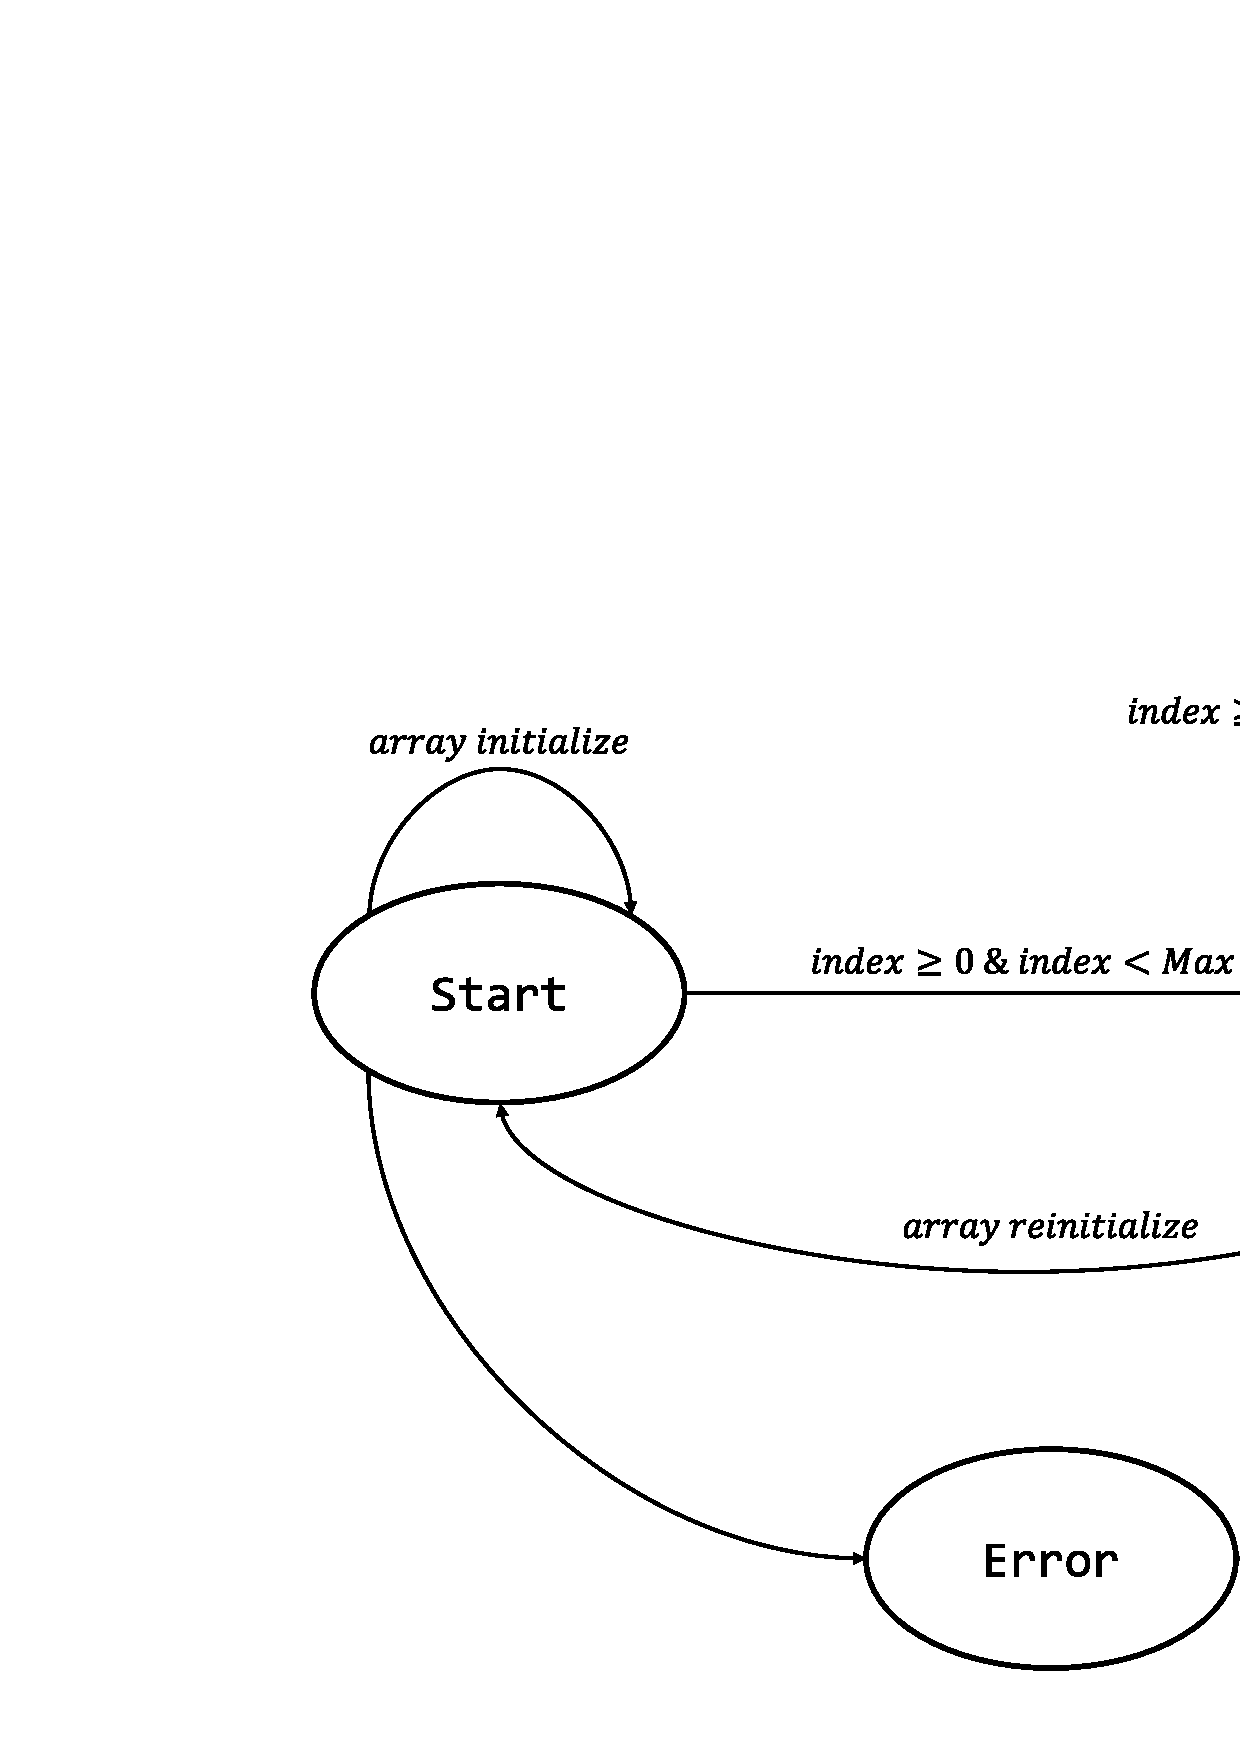
\includegraphics[scale = .25]{images/ArrayIndex.pdf}
\caption{array index out of bound formulated as FSM}
\label{fig:array}
\end{figure}


We can visualize all runtime exceptions as finite state machine (FSM). When a
program violates such sequence, it throws runtime exception. 
In Figure~\ref{fig:array}, array index out of bound (java.lang.
ArrayIndexOutOfBoundException) exception is described as a FSM. 
Here, a program will be in safe bound as long as the $array\_index \geq 0$ or
$array\_index \leq max\_array\_size - 1$

\subsection{Constraint Automata}
\label{subsec:constraintAutomata}

\emph{Constraint automata} is a formalism to describe the behavior and possible
data flow in coordination models. 
Mostly used for model checking. We have used it for the purpose of program
repairing technique. Here we define the finite state automata as follows :

$$(Q, \Sigma, \delta, q_0, F)$$
\begin{mybullet}
 \item $Q$: set of state where $|Q| = 2$, \emph{legal state}(init) and
\emph{illegal state} (error).
 \item $\Sigma$: symbols, invariants based on exception type.
 \item $\delta$: transition function. $init \rightarrow init$ is safe
transition and $init \rightarrow error$ is the invariant violation.
 \item $q_0$: starting state, here $q_0 = init$.
 \item $F$: end state, here it same as $q_0$.
\end{mybullet}

\begin{figure}[t]
\centering
\includegraphics[scale=.25]{images/automata.pdf}
\caption{Constraint automata general model}
\label{fig:automata}
\end{figure}

According to the Figure~\ref{fig:automata}, the repairing mechanism will only
trigger when we have a transition from 
init state to error state due to invariant violation.

\subsection{Patching Techniques}
\label{subsec:patchCA}

The patching technique is based on the exception type. 

\section{Repairing Strategy: Exception Type}
\label{sec:strgEx}

%marker
%textcolor{red}{\textbf{Please review this section}}\newline

\begin{figure}[t]
\lstset{language=Java, caption=Java code which may throws runtime exceptions,
label=example1}
\begin{lstlisting}[countblanklines=false]
public class TestClass {
    private int[] arr1;
    private int[] arr2;
    private int[] arr3;

    public TestClass(int[] arr1, int[] arr2, int[] arr3) {
	this.arr1 = arr1;
	this.arr2 = arr2;
	this.arr3 = arr3;
    }
    public int[] fun(int a, int b, int c, int d) {
	int temp0 = a + b;
	int temp1 = c * d;
	int temp2 = temp0 - temp1;
	//array index out of bound, negative index
	int temp3 = this.arr1[temp0];
	//array index out of bound, negative index
	int temp4 = this.arr2[temp1];
	//array index out of bound, negative index
	int temp5 = this.arr3[temp3];
	int temp6 = temp4 + temp5;
	int temp7 = temp6 - temp3;
	//array index out of bound, negative index, divide by zero
	this.arr1[temp6] = temp7/(d-a);
	//array index out of bound, negative index, divide by zero
	this.arr2[temp7] = temp7/temp4;
	if(arr2[temp1] ! = arr3[temp7]) return arr1;
	else return null;
    }
}
public class MainClass {
    public void main(String[] a) {
	int[] arr1 = {1,2,3,4};
	int[] arr2 = {1,2,3,4};
	int[] arr3 = {1,2,3,4};
	TestClass TC = new TestClass(arr1, arr2, arr3);
	int[] res = TC.fun(2,4,3,4);
	//Null pointer exception
	System.out.print("Result : "+res[2]);
    }    
}
\end{lstlisting}
\end{figure}

In the Example~\ref{example1}, we have given a piece of \java\ code which shows
multiple lines can throw several runtime exceptions.
In this example we consider three very common runtime exceptions:
NullPointerException, ArrayIndexOutOfBoundExcepltion, NegetiveIndexException,
ArithmeticException (i.e. divide-by-zero). In rest of this section, this
particular example will be used to demonstrate the repairing strategy.

\subsection{Symbolic Analysis}
\label{subsec:symb}

\begin{figure}[t]
\centering
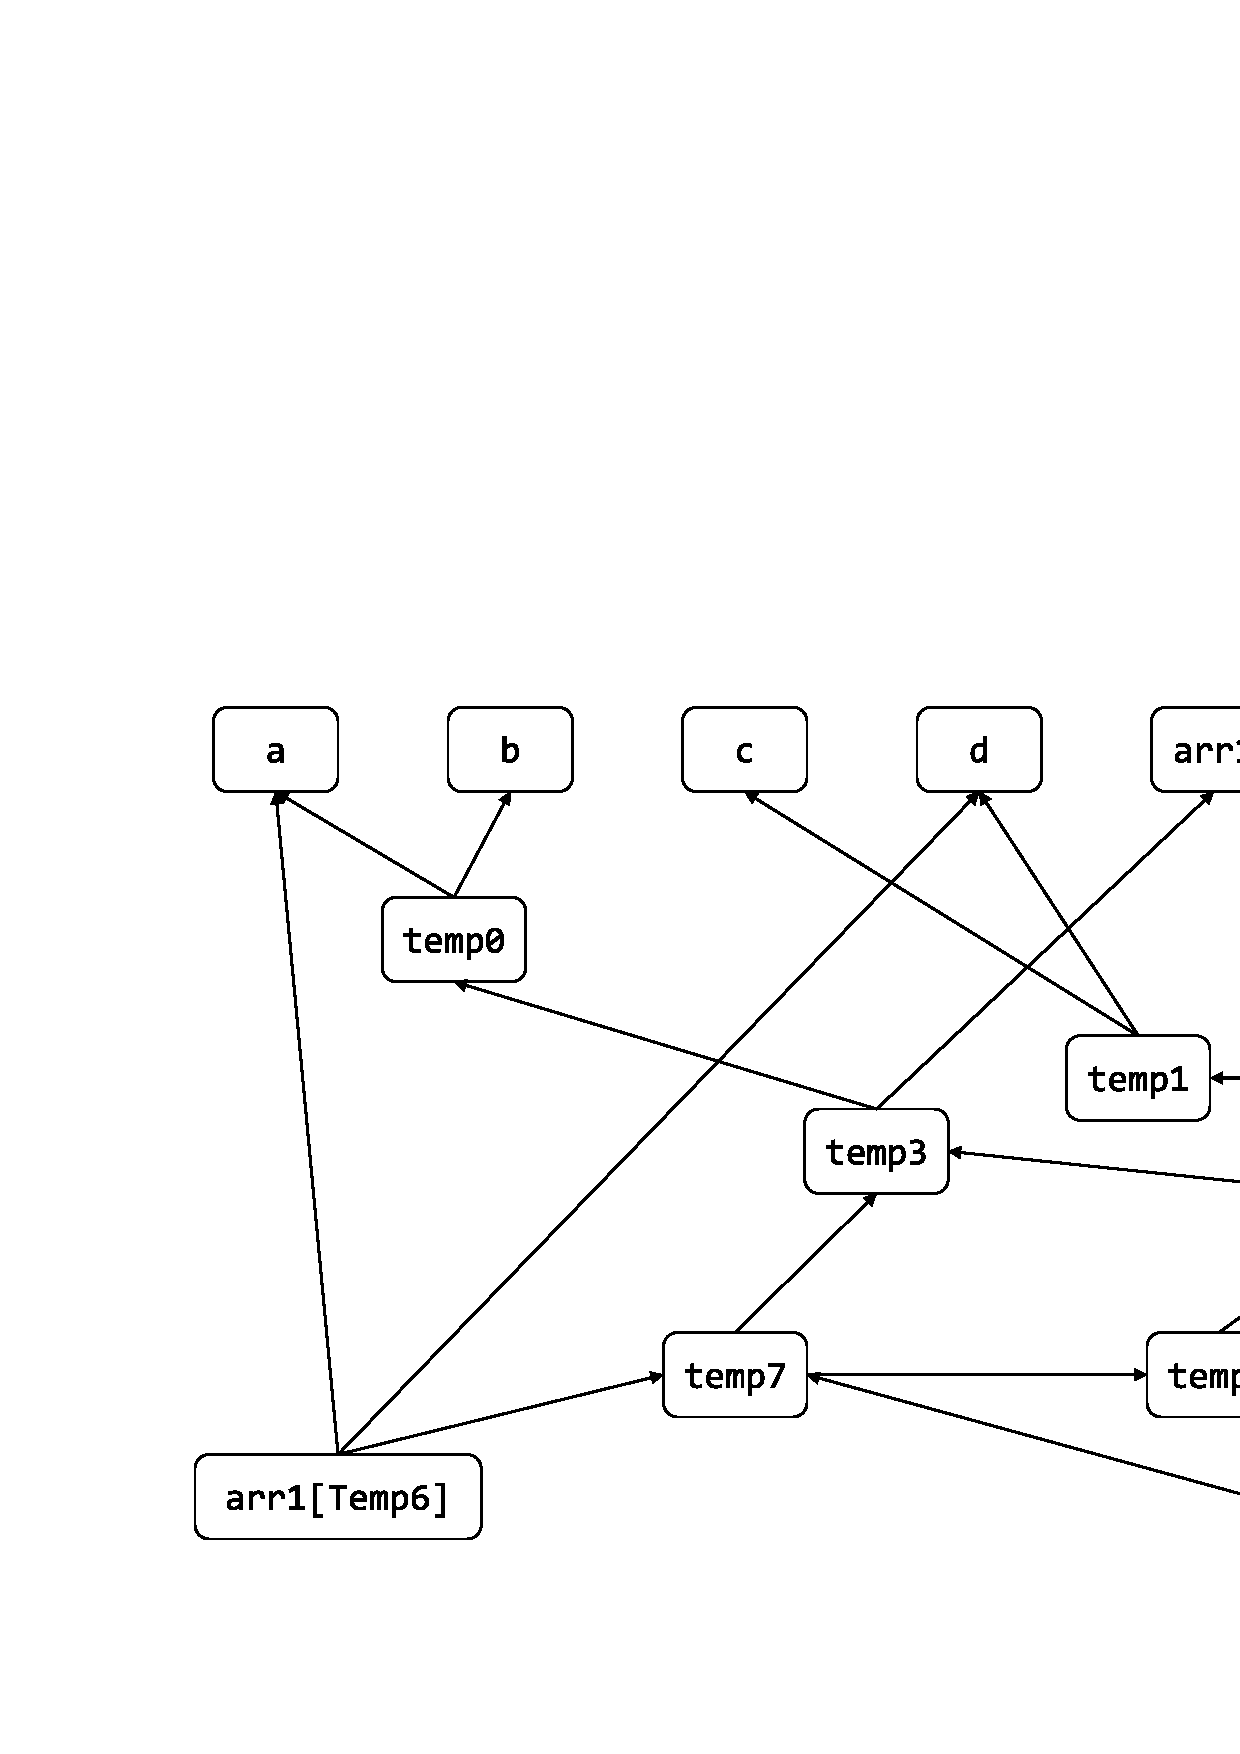
\includegraphics[width=3.3in]{images/depG.pdf}
\caption{Data dependency graph of the variables in Example\ref{example1}}
\label{fig:datadep}
\end{figure}

We have done several  static analysis a priori  over the Java source code to
discover :
\begin{mylist}
\item Critical section of the code which are not eligible for patching. Eg.
banking or any financial transaction which should be crashed in case of
exception as suboptimal solution due to patching will led it to inconsistent
state.
\item Symbolic analysis of the program to discover potential points of failure
and mark them.
\item Build data dependency graph which will be used to generate appropriate
code slice to be used as patch.
In Figure~\ref{fig:datadep}, the data dependency graph of the example
code~\ref{example1} is presented.
\item The symbolic analysis will also reveal which kind of exception is likely
to happened at the time of execution.
This information is necessary at the time of instrumenting the patch as it will
determine the catch block.
	
\end{mylist}

\subsection{Data set for Successful Program Runs}
\label{subsec:progrun}

Here we will store all the traces of successful program runs.
\begin{figure}[t]
\centering
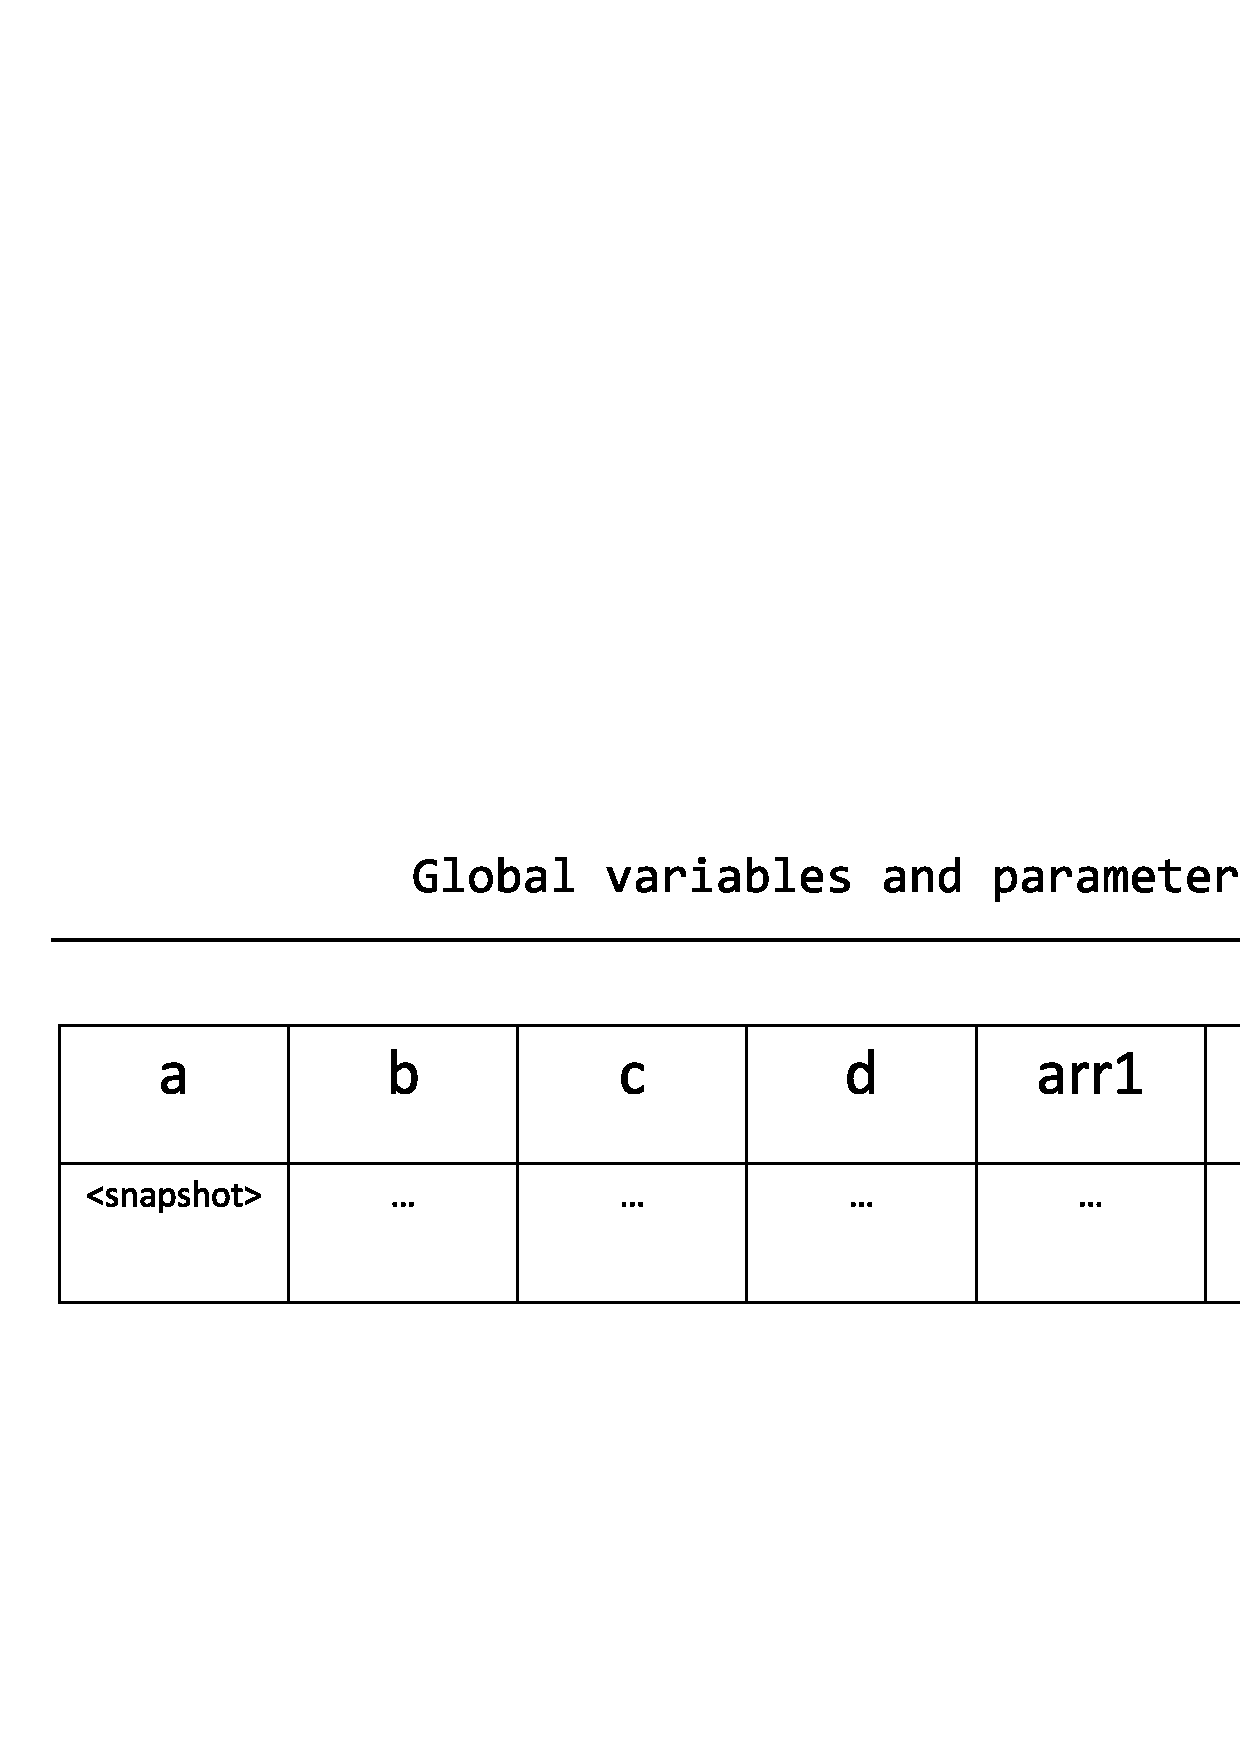
\includegraphics[width=3.0in]{images/succrun.pdf}
\caption{Indexed global variables and method arguments successful runs}
\label{fig:succrun}
\end{figure}

Figure~\ref{fig:succrun} shows such indexed traces of all the global variables
and method arguments.
We store the snapshots of these objects. We won't store local variables as they
can always be regenerated.
As it is required to capture the snapshot of all these variable, we made deep
cone of all of these objects and variables.

% begin{table}[htb]
%\begin{tabular}{|c|c|c|c|c|c|c|}
%\hline
%a & b & c & d & arr1 & arr2 & arr3 \\ \hline
%\ldots & \ldots & \ldots & \ldots &	\ldots & \ldots & \ldots\\ \hline
%\end{tabular}
%\caption{Trace of successful runs}
%	\label{tab:Trace}
%\end{table}


\subsection{Matrices}
\label{subsec:martices}

%marker
%\textcolor{red}{\textbf{Please review this section.}}\newline

\subsection{Instrumenting Patching}
\label{subsec:patchinstru}

We have used Soot framework which is a Java byte code manipulator to instrument
patch. 
The patching technique is divided into two phases

\subsubsection{Determine Exception Type} 

At the time of execution, the exception may happened due to some specific values
of some variables. We will catch the exception. Here the type of runtime
exception is $java.lang.ArrayIndexOutOfBound$. This will be used to produce the
try-catch block.
 
\subsubsection{Determine Optimal Code Slice}

The optimal code slice will be determined from the data dependency graph which
was rendered at the time of static analysis mentioned in
\S~\ref{subsec:symb}. In the Listing~\ref{patchingexample1}, the example
code snippet shows such code slice inside the catch block.
As the error occurred at the line $int\ temp5\ =\ this.arr3[temp3];$ the
statements which produces the temp3 and the statement which also involves
$temp3$ or any other variables derived from $temp3$, would be included in the
catch block for re-execution with the valued of the same from the data table of
previous successful runs.

 

\lstset{language=Java, caption=patching code slice based on exception type,
label=patchingexample1}

\begin{figure}[t]
\begin{lstlisting}[countblanklines=false]
public class TestClass {
    private int[] arr1;
    private int[] arr2;
    private int[] arr3;

    public TestClass(int[] arr1, int[] arr2, int[] arr3) {
	this.arr1 = arr1;
	this.arr2 = arr2;
	this.arr3 = arr3;
    }
    public int[] fun(int a, int b, int c, int d) {
	try {
	    int temp0 = a + b;
	    int temp1 = c * d;
	    int temp2 = temp0 - temp1;
	    int temp3 = this.arr1[temp0];
	    int temp4 = this.arr2[temp1];
	    //IndexOutOfBoundException as temp3 = 20
	    int temp5 = this.arr3[temp3];
	    int temp6 = temp4 + temp5;
	    int temp7 = temp6 - temp3;
	    this.arr1[temp6] = temp7/(d-a);
	    this.arr2[temp7] = temp7/temp4;
	} catch(IndexOutOfBoundsException indEx) {
	    int temp0 = a + b;
	    int temp1 = c * d;
	    int temp2 = temp0 - temp1;
	    int temp3 = this.arr1[temp0];
	    //Bellow line is not part of the patch as
	    //temp1 and temp3are not related to temp3
	    //for which the exception occurred.
	    //int temp4 = this.arr2[temp1];
	    int temp5 = this.arr3[temp3];
	}
	if(arr2[temp1] ! = arr3[temp7]) return arr1;
	else return null;
    }
}
public class MainClass {
    public void main(String[] a) {
	int[] arr1 = {20,21,22,23};
	int[] arr2 = {1,2,3,4};
	int[] arr3 = {10,11,12,13};
	TestClass TC = new TestClass(arr1, arr2, arr3);
	int[] res = TC.fun(2,4,3,2);
	System.out.print("Result : " + res[2]);
    }    
}
\end{lstlisting}
\end{figure}

\subsection{Variable Tracking and Monitoring}
\label{subsec:taint}
%\textcolor{red}{\textbf{I have added standard taint analysis technique here as
%an example. We can change it later}}\newline


Here we used taint analysis technique to tag variables and objects of our
interest to monitor them.
This steps are necessary as the values of the variables used during the
instrumentation may cause further runtime exceptions.
We used bit-vector which is an efficient technique to taint a object/variable.
It requires maintain a single dimension byte array where each bit correspond to
a single object/variable of our interest.
The bit values will be flipped when it is required to taint ($1$) or untaint
($1$) an object/variable.
We will only monitor these entities until all of them flushed from the program
and the entire program reached to a stable state.
\section{Repairing Strategy : Constraint Automata}
\label{sec:strgCA}

\subsection{General Structure}
\label{subsec:generalCA}

\emph{Constraint automata} is a formalism to describe the behavior and possible data flow in coordination models. 
Mostly used for model checking. We have used it for the purpose of program repairing technique. Here we define the finite state automata as follows :

$$(Q, \Sigma, \delta, q_0, F)$$
\begin{itemize}
	\item $Q$: set of state where $|Q| = 2$, \emph{legal state}(init) and \emph{illegal state} (error).
	\item $\Sigma$: symbols, invariants based on exception type.
	\item $\delta$: transition function. $init \rightarrow init$ is safe transition and $init \rightarrow error$ is the invariant violation.
	\item $q_0$: starting state, here $q_0 = init$.
	\item $F$: end state, here it same as $q_0$.
\end{itemize}

\begin{figure}[!htb]
\centering
\includegraphics[width=3.2in]{images/automata.eps}
\caption{Constraint automata general model}
\label{fig:automata}
\end{figure}

According to the Figure~\ref{fig:automata}, the repairing mechanism will only trigger when we have a transition from 
init state to error state due to invariant violation.

\subsection{Patching Techniques}
\label{subsec:patchCA}

The patching technique is based on the exception type. 

\subsubsection{Array index out of bound exception}

Array index out of bound exception happen when one tries to access the array with a index which is more than the size of the array or 
less than zero i.e. with some negative value. We did the patching based on these two scenario. When the index is more than the array size, 
we patch it by assigning $array.length - 1$.

\lstset{language=Java, caption=array index out of bound patching, label=patchingexample2}

\begin{lstlisting}
void foo()
{
  int []arr = {1,2,3,4};
  int index = 10;
  int y = 0;
  try
  {
    //original code
    y = arr[index];
  }
  //patching instrumentation
  catch(IndexOutOfBoundException ex)
  {
    if(index > arr.length)
      y = arr[arr.length - 1];
    else
      y = a[0];
  }
}

\end{lstlisting}

\subsubsection{Negative Array Size Exception}

Negative array size exception occurs when one tries to create a array with a negative size. 
The patching is done based on data flow analysis. Suitable index size is determined by looking at the successive statement dependent on the array. 
To take a safe bound, we took maximum index size and set as the array size in the new array statement.


\lstset{language=Java, caption=arr index out of bound patching, label=patchingexample2}

\begin{lstlisting}
void foo()
{
  int []arr = {1,2,3,4};
  int index = 10;
  int y = 0;
  try
  {
    //original code
    y = arr[index];
  }
  //patching instrumentation
  catch(IndexOutOfBoundException ex)
  {
    if(index > arr.length)
      y = arr[arr.length - 1];
    else
      y = a[0];
  }
}

\end{lstlisting}

\subsubsection{Arithmetic Exception : Division-by-zero Exception}

Division by zero causes arithmetic exception. There are two different cases which were considered here. 
\begin{itemize}
	\item \textbf{Case I :} The denominator is going to the taint sink but the left hand side is not going to any taint sink. 
	Here we will not manipulate the denominator as we are not manipulating any variable which are going to any taint sink.
	\item \textbf{Case II :} The denominator and the left hand side, both are not going to any taint sink. So they are safe to patch.
\end{itemize}

\lstset{language=Java, caption=arithmetic exception : division-by-zero patching, label=patchingexample2}

\begin{lstlisting}
void foo()
{
  int a = 10;
  int b = 0;
	int y;
  try
  {
    //original code
    y = a/b;
  }
  //patching instrumentation
  catch(ArithmeticException ex)
  {
    //case I
    if(taintSink(b))
      y = 0;
    //case II
    else
    {
      b = 1;
      y = a/b;
    }
  }
}
\end{lstlisting}

\subsubsection{Null Pointer Exception}

Null pointer exception in Java is the most common runtime exception encountered. 
Thrown when an application attempts to use null in a case where an object is
required. There exists various scenarios where null pointer exception can
happen. These different scenario requires different patching techniques. Bellow
we enlist all cases and corresponding patching techniques.


\begin{itemize}
  \item \textbf{Case I} Calling the instance method of a null object. \newline
  \textbf{Patch :} This is patched by calling the constructor. In case there
  exists more than one constructor then we need to find most appropriate
  constructor. This is done by using data flow analysis in the successive
  statement to see which fields/methods been accessed and according to that
  most suitable constructor should be picked up, this will ensure safest way to
  deal with the later method calls/field accesses.
  
  \lstset{language=Java, caption=appropriate constructor, label=patchingexample2}

\begin{lstlisting}
class MyClass
{
 Integer field1;
 String field2;
 Double field3;

 public MyClass()
 {
  this.field1 = 1;
  this.field2 = null;
  this.field3 = null;
 } 
 public MyClass(Integer field1, String field2)
 {
  this.field1 = field1;
  this.field2 = field2;
  this.field3 = null;
 } 
 public MyClass(Integer field1, String field2, Double field3)
 {
  this.field1 = field1;
  this.field2 = field2;
  this.field3 = field3;
 }
 public Double getfield3()
 {
  return this.field3;
 }
}

class main
{
 Myclass mclass = null;
 Double a = null;
 try
 {
  //original code
  a = mclass.getfiled3() + 5.0;
 }
 //instrumentation
 catch(NullPointerException ex)
 {
  //choose appropriate constructor
  mlass = new MyClass(1, "a", 1.0); 
  a = mclass.getfiled3();
 }
}
\end{lstlisting}
  \item 
  
  \item \textbf{Case II} Possible Accessing or modifying the field of a null
  object.\newline
  \textbf{Patch :} The patch is same as the previous one.
  
  \item \textbf{Case III} Taking the length of null as if it were an
  array.\newline
  \textbf{Patch :}The patch for this situation is very much similar to the
  negative array size exception. Here we will do a data-flow analysis to see all
  the successive statements where the array object has been used (read or
  write). For safety we will take the maximum index from those statements and
  reinitialize the array object with the size.
    
  \lstset{language=Java, caption=array null pointer exception,
  label=patchingexample2}

\begin{lstlisting}
int[] bar(int a)
{
 int []arr = new int[a];
 int []b = (a > 10) ? arr:null;
 return b; 
}
void foo()
{
 int[] arr;
 int []arr = bar(5);
 try
 {
  //access or modify any field of arr
  //this will throw a null pointer exception
 }
 //instrumented code
 catch
 {
  int ARRAY_SIZE = 11;
  int []arr = new int[ARRAY_SIZE];
  //access or modify any field of arr
 }
}
\end{lstlisting}

  \item \textbf{Case IV} Accessing or modifying the slots of null as if it were
  an array.
 \textbf{Patch :} The patching mechanism is exactly same as before.
 
  \item \textbf{Case V} Throwing null as if it were a Throwable value.
\end{itemize}



%%%%%%%%%%%%%%%%%%%%%%%%%%%%%%%%%%%%%%%%%%%%%%%%%%%%%%%%%%%%%%%%%%%%%%%%%%%%%%%%%%%%%%%%%%%
%%%%%%%%%%%%%%%%%%%%%%%%%%%%%%%%%%%%%%%%%%%%%%%%%%%%%%%%%%%%%%%%%%%%%%%%%%%%%%%%%%%%%%%%%%%

\section{Design of the System}
\label{sec:SystemDesign}


%later convert this pdf
\begin{figure}[t]
\centering
\includegraphics[width=3.2in]{images/OverallDesign.png}
\caption{Overall Design}
\label{fig:overallDesign}
\end{figure}


% \begin{figure}[!htb]
% \centering
% 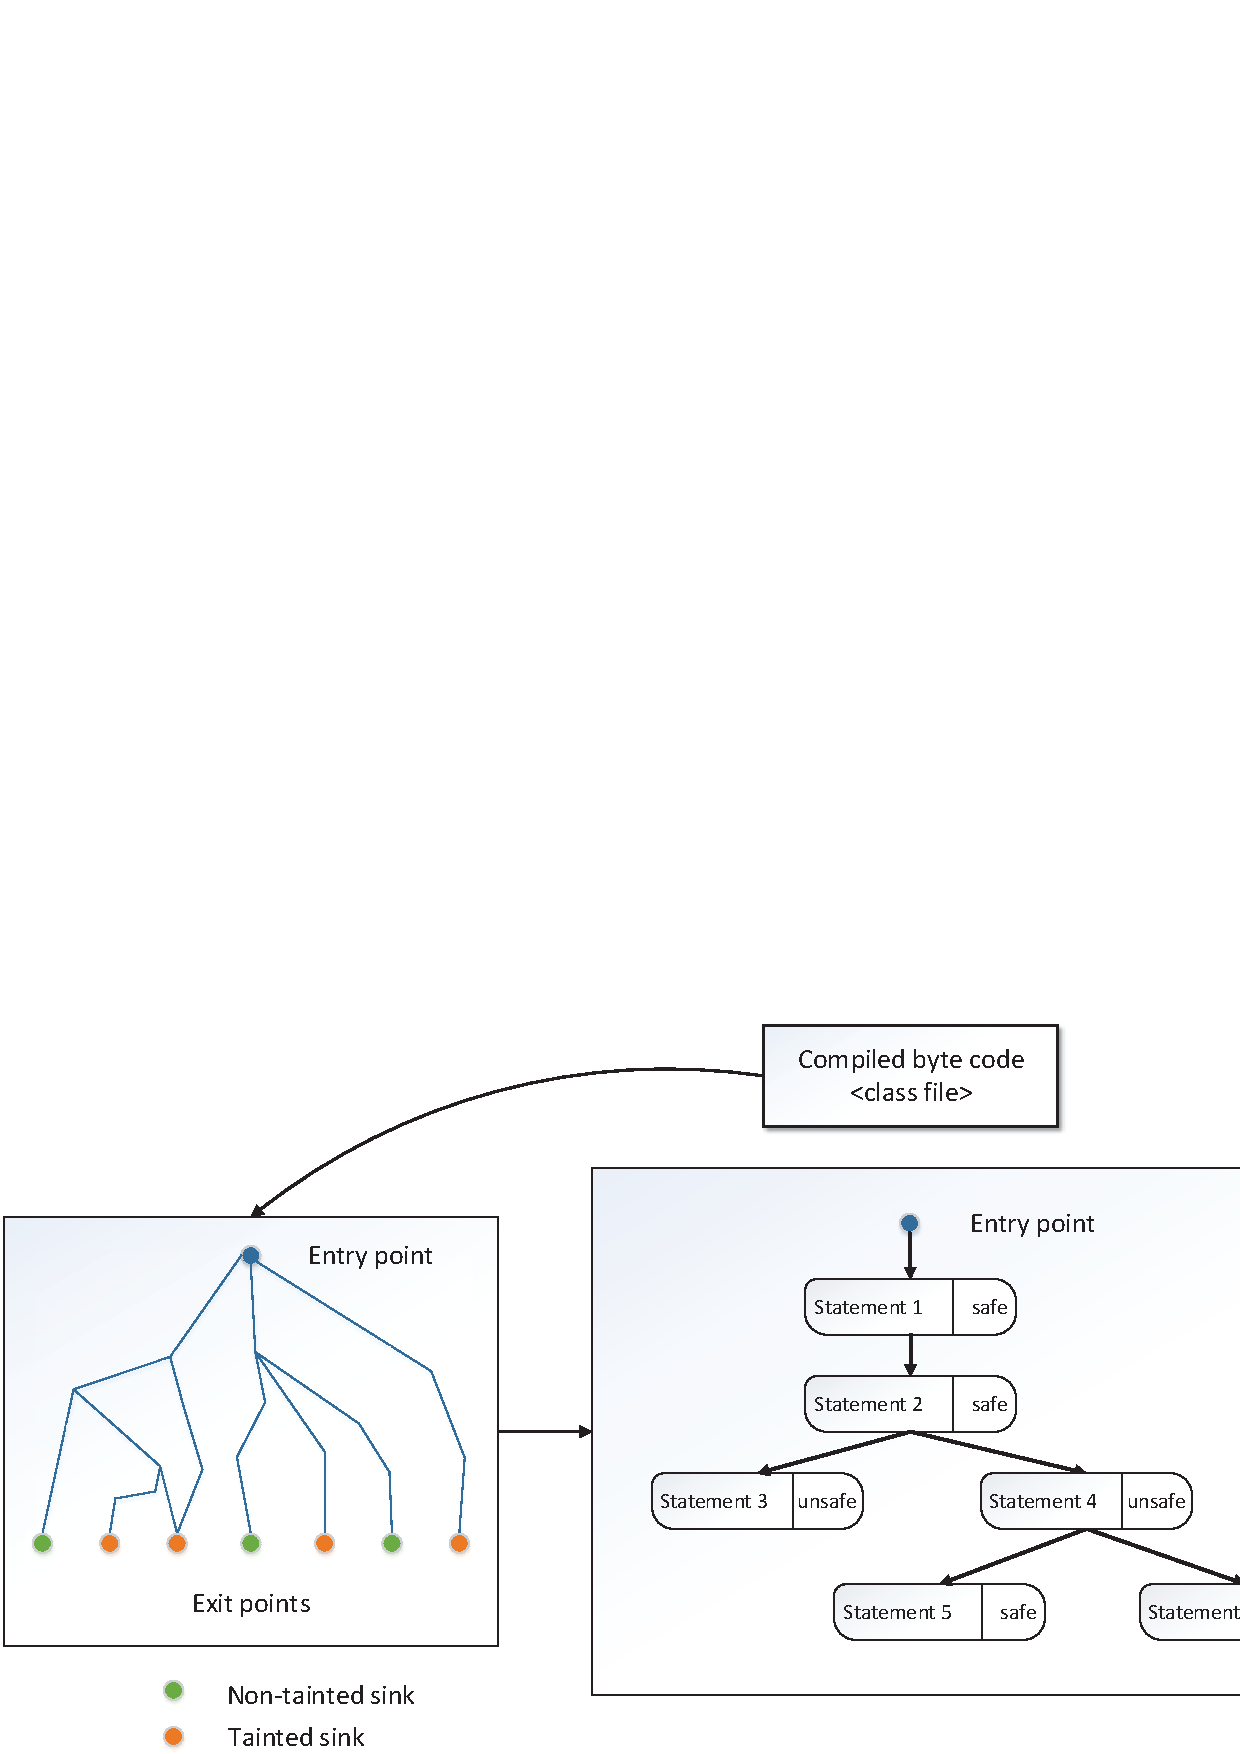
\includegraphics[width=3.5in]{images/TaintModule.pdf}
% \caption{Overall Design}
% \label{fig:TaintModule}
% \end{figure}
% 
% \begin{figure*
%   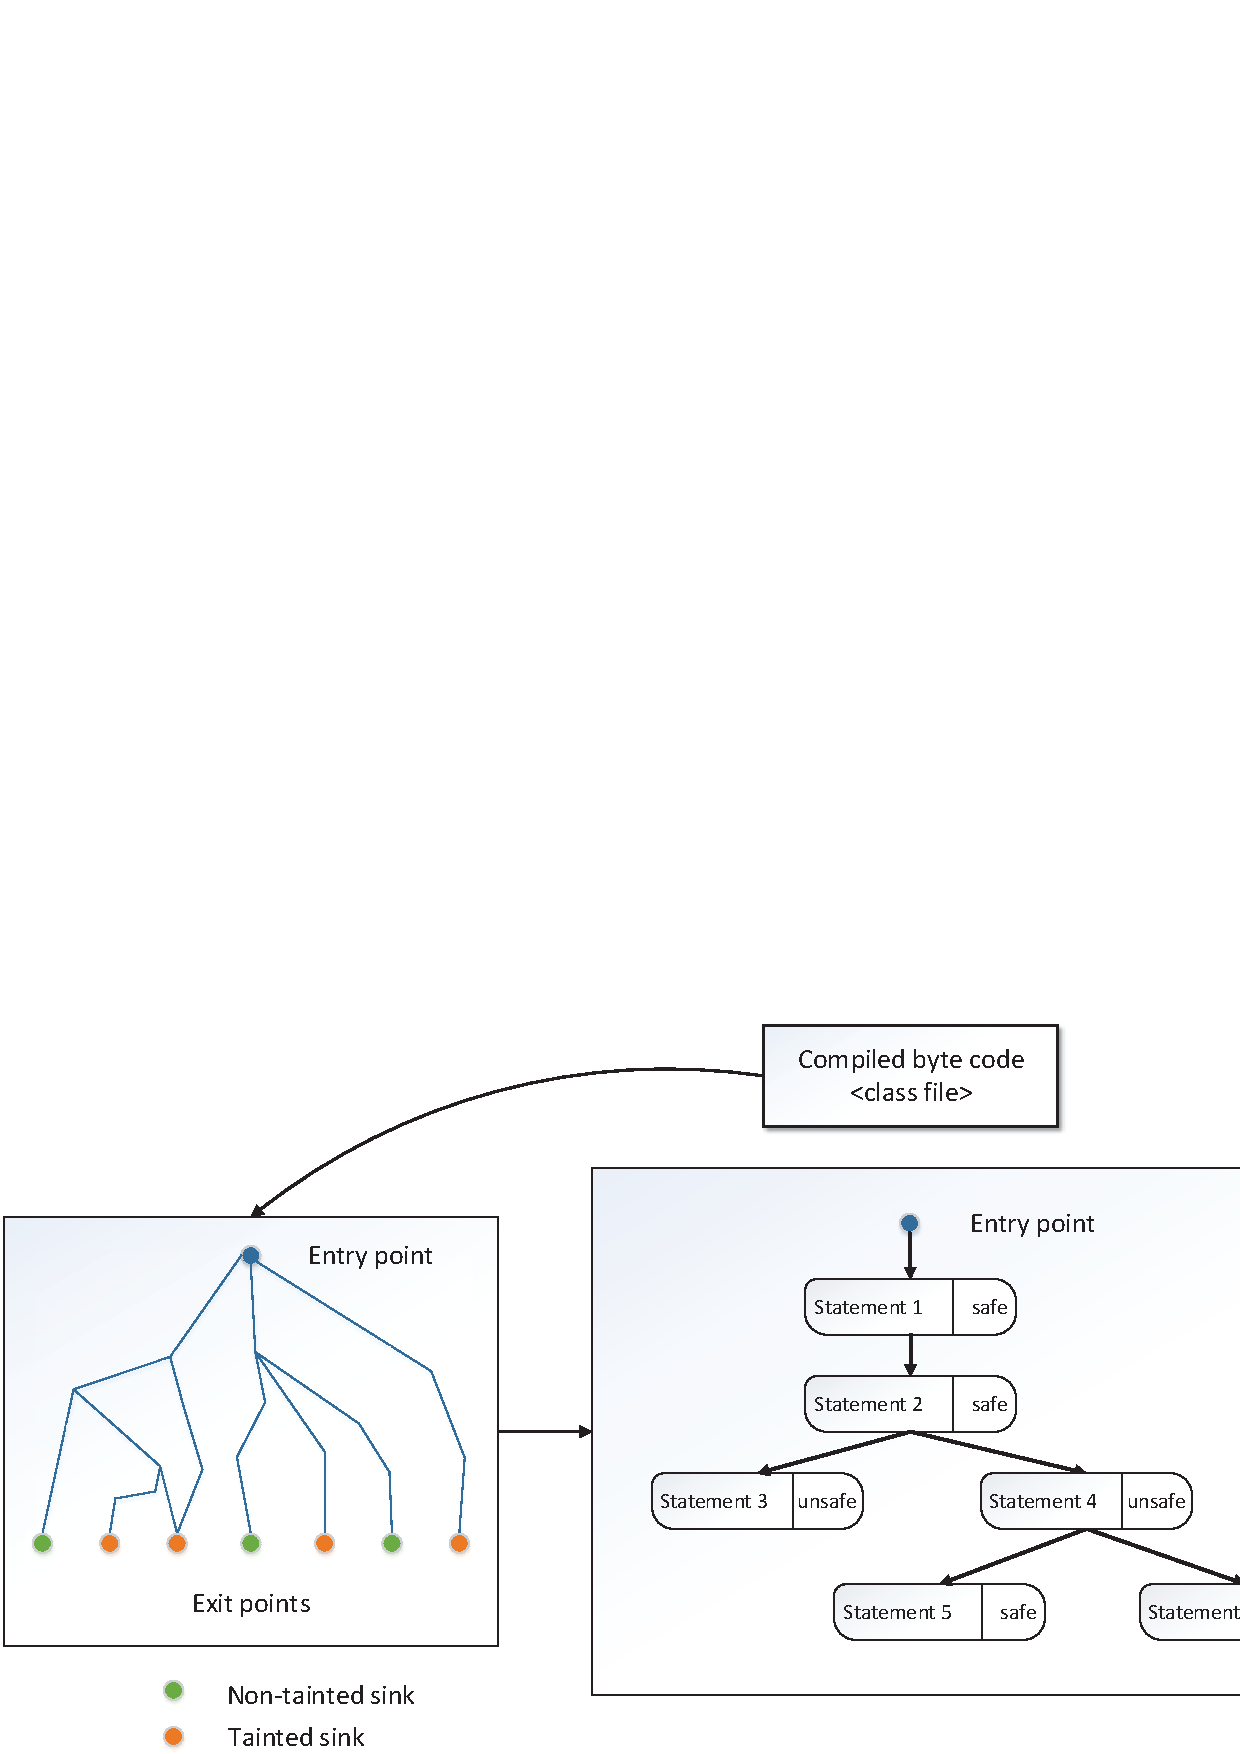
\includegraphics[width=\textwidth,height=5cm]{images/TaintModule.pdf}
%   \caption{Design of the Taint Module}
% \end{figure*}

%later covert this to pdf
\begin{figure*}[t]
\centering
  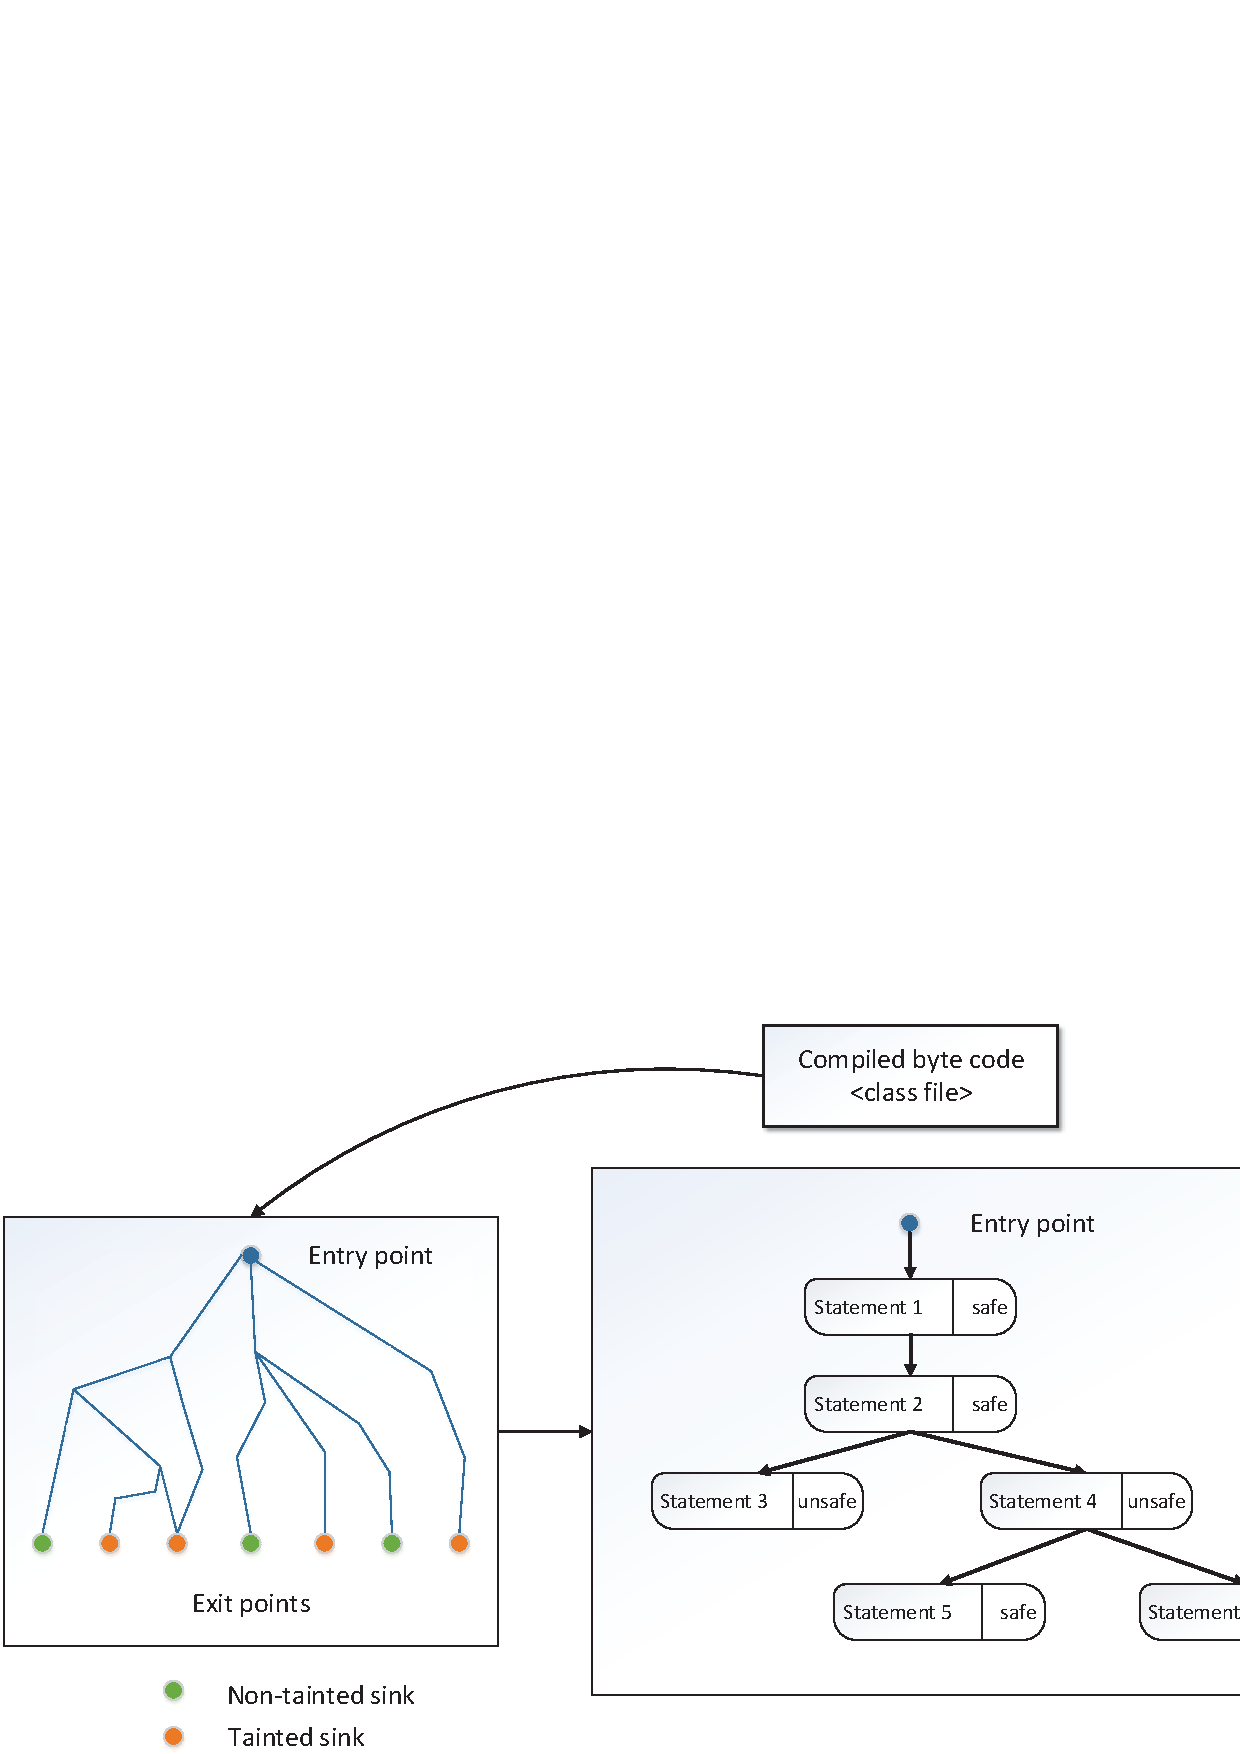
\includegraphics[width= 7.0in]{images/TaintModule.png}
  \caption{Design of the Taint Module}
  \label{fig:TaintModule}
\end{figure*}


The overall design of the repairing framework is illustrated in
Figure~\ref{fig:overallDesign}. The framework consists of two basic modules.


\subsection{Taint analysis Module}
\label{subsec:TaintModule}

The main purpose of the taint analysis module is to classify which of the
statements are safe to patch or not. Based on the analysis result in this
module, the tagged statement will be passed to the repairing module.


We have specify the list of source, sink and derivation methods in a
configuration file before the analysis. The source methods includes methods
which
take input from user from console or web application forms like text box. The
sink methods are sensitive data storage which are unsafe to manipulate such as
database, console print or methods to send a text file to printer etc. The
overview of the taint analysis module is illustrated in the
Figure~\ref{fig:TaintModule}.  The input for the module is the compiled byte
code intended to be repaired. Here we have generated a control flow graph (CFG)
from the class file to get all the possible program paths. Here a point to be
noted that any modification along the path going to the tainted sink is unsafe
to patch.


\subsubsection{Tainting Rules}
\label{subsubsec:TaintingRule}
%\textcolor{red}{\textbf{Needs Revision}}\newline

\begin{table}[t]
\centering
\small
\begin{tabular}{l|l}
\multicolumn{1}{c|}{\textbf{\java\ Class}} & \multicolumn{1}{c}{\textbf{Source
Method}}\\
% \scalebox{0.86}
% {
\hline
\code{java.io.InputStream} & \code{read()}\\
\code{java.io.BufferedReader} & \code{readLine()}\\
\code{java.net.URL} & \code{openConnection()}\\
\code{org.apache.http.HttpResponse} & \code{getEntity()}\\
\code{org.apache.http.util.EntityUtils} & \code{toString()}\\
\code{org.apache.http.util.EntityUtils} & \code{toByteArray()}\\
\code{org.apache.http.util.EntityUtils} & \code{getContentCharSet()}\\
\code{javax.servlet.http.HttpServletRequest} & \code{getParameter()}\\
\code{javax.servlet.ServletRequest} & \code{getParameter()}\\
\code{java.Util.Scanner} & \code{next()}\\
\end{tabular}
\caption{Common \java\ library taint source functions}
\label{tab:TaintSources}
% }
\end{table}



\begin{table}[t]
\centering
\small
\begin{tabular}{l|l}
\multicolumn{1}{c|}{\textbf{\java\ Class}} & \multicolumn{1}{c}{\textbf{Sink
Method}}\\
% \scalebox{0.86}
% {
\hline
\code{java.io.PrintStream} & \code{printf()}\\
\code{java.io.OutputStream} & \code{write()}\\
\code{java.io.FileOutputStream} & \code{write()}\\
\code{java.io.Writer} & \code{write()}\\
\code{java.net.Socket} & \code{connect()}\\
%org.apache.http.impl.client.DefaultHttpClient & execute\\ \hline
\end{tabular}
% }
\caption{Common \java\ library taint sink functions}
\label{tab:TaintSinks}
\end{table}


We have used extended InFlow framework for the taint analysis module. The steps
are

\begin{mylist}
  \item We defined list of source and sink taint methods listed in
  Table~\ref{tab:TaintSources} and \ref{tab:TaintSinks}. We are only tainting
  the variables which are coming from the listed taint source methods.
  
  \item We have also listed all taint propagation methods. The assignment ($=$)
  is the basic taint propagator. But there are other methods like \code{append}
  in \code{java.lang.StringBuffer} and \code{java.lang.StringBuilder} which are
  taint propagator.

  \item All the variable which are referred to tainted variables/ objects or
  output of taint propagator over tainted variable/objects are also considered
  as tainted.

  \item For all the program patch we see if such tainted variables are reaching
  the tainted sink or not. If they are reaching to some tainted sink then all
  the statements along that particular program path to which the tainted
  variables are assigned are marked as unsafe otherwise safe.
\end{mylist}


\subsection{Repairing Module}
\label{subsec:RepairingModule}

%later covert this to pdf
\begin{figure}[t]
\centering
  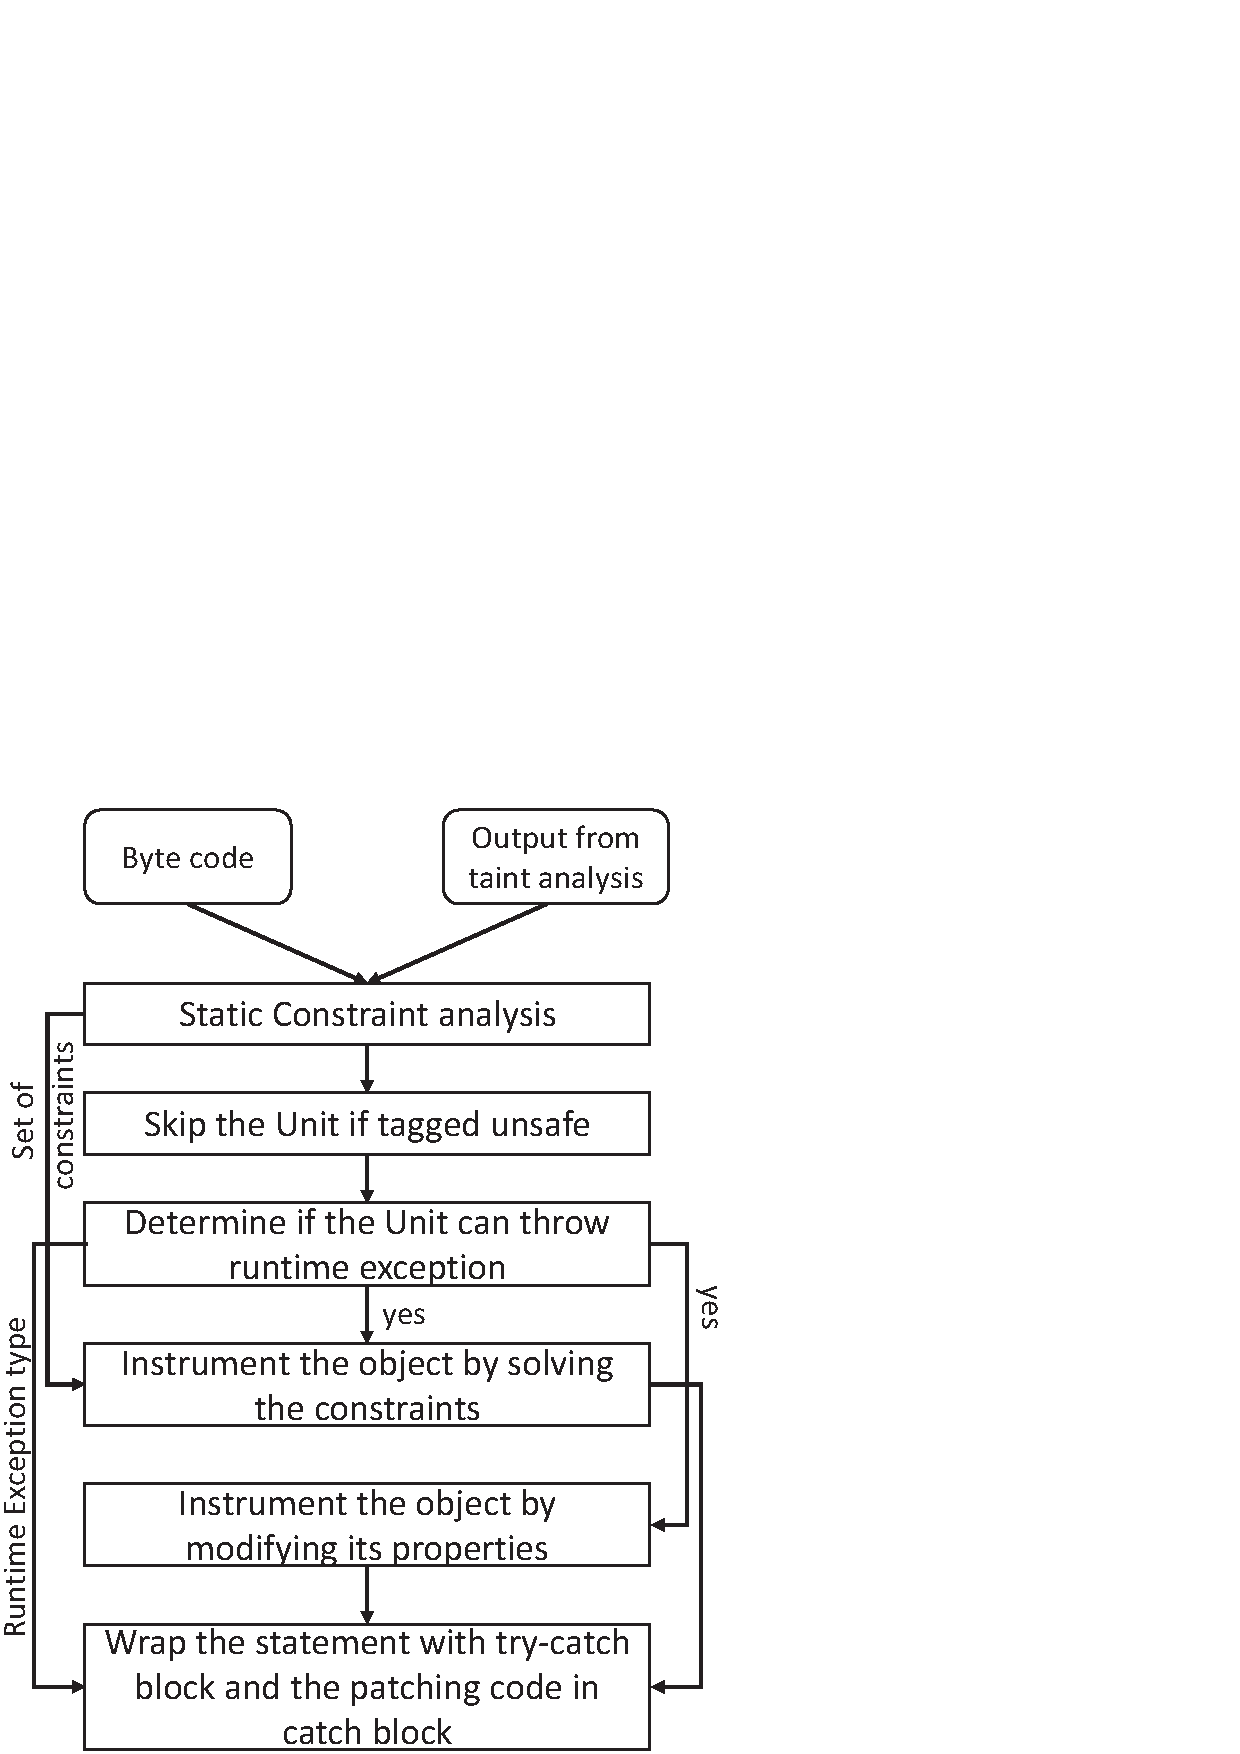
\includegraphics[scale= .5]{images/PatchModule.png}
  \caption{Design of the Patching Module}
  \label{fig:PatchModule}
\end{figure}

The repairing module is consisted of three phases. All these three phases
requires three sequential passes over the input bytecodes to produce the final
patched result.


\subsubsection{Method Shilding}
\label{MethodShilding}


When we are shielding a method, we also looked to the calling context of that
particular method. The method can be called from a path which leads to some
tainted sink and it can also be called from such path which does not contain
any taint sink. In such cases, we have taken special care about the callee. The
path to the tainted sink should not call a patched method as it can influence
data which are leaving the system. So, we also maintained two different version
of
the method and instrument the calling site so that appropriate method is called.

\lstset{language=java, caption = Same method calling in different scenario,
label=callingContext}
\begin{figure}[t]
\begin{lstlisting}[countblanklines=false]
int bar(int a, int b) {
    return a/b;
}
void foo() {
    int a = 10, b = 0, c = 15;
    int out = bar(a, b);
    TaintSink(out);
    int out1 = bar(c, b);
    NonTaintSink(out1);
}
\end{lstlisting}
\end{figure}

\lstset{language=java, caption = Method name modification for different calling
context, label=callingContextPatch}
\begin{figure}[t]
\begin{lstlisting}[countblanklines=false]
int bar(int a, int b) {
    return a/b;
}
int bar_untainted_fa844d57(int a, int b) {
    int out;
    try {
	out = a/b;
    } catch(ArithmeticException ex) {
	b = 1;
	out = a/b;
    }
    return out;
}
void foo() {
    int a = 10, b = 0, c = 15;

    // no modification in the call where the result can go to a tainted sink
    // method
    int out = bar(a, b);
    TaintSink(out);

    // Modify the method call to the shielded method as the result is not going
    // to any tainted sink method
    int out1 = bar_untainted_fa844d57(c, b);
    NonTaintSink(out1);
}
\end{lstlisting}
\end{figure}

In the Listing~\ref{callingContext} and \ref{callingContextPatch} we have
defined an example code snippet of the original code and the patched code where
we have renamed the method \emph{bar} to \emph{bar\_untainted\_fa844d57}
before instrumenting any patching code in it. The variable \emph{out} goes to a
tainted sink while \emph{out1} does not. So the we have done modification in the
line where \emph{out1} is defined. As \emph{out} is going to a tainted sink
method, we did not do any modification to it.



% \begin{enumerate}
%   \item \textbf{Taint analysis module :}
%   \item \textbf{Repairing Module : }
% \end{enumerate}


\section{Benchmark Results}
\label{sec:bench}
\section{Related Work}
\label{sec:relatedWork}

There has been considerable amount of research done in the area of automated
program repairing. The approaches that have been proposed by the researchers
broadly fall into two categories namely, static and dynamic.

The static approaches work based on the counter-example or the violated
invariants that are reported from the field. These approaches then repair the
program by automatically developing a patch and then ensure its correctness
using computationally intensive techniques such as model-checking
\cite{biere2014, wei-issta-2010}.
These techniques are effective in producing accurate patches. However, shutting
down the system to produce and apply patches is not always feasible or
desirable. To overcome these problems, several promising dynamic approaches have
been proposed. These approaches typically develop either suboptimal patches or
isolate the data structure that is damaged which allows at least part of the
system to be functional \cite{conf/issre/DemskyR03, conf/icse/DemskyR05,
conf/issta/DemskyEGMPR06}. The advantage of these approaches is that they are
light-weight and can fix the system on-the-fly. Long et al.
\cite{conf/pldi/LongSR14} have developed an approach that deals with two most
commonly observed software errors, and then suppressing the errors with the help
of a runtime that operates by first invoking a  signal handlers, and then by
running a dynamic symbolic execution to ensure no side-effects.
This approach is light-weight and like our approach fixes the errors on-the-fly
potentially allowing some sub-optimal behaviour for a finite time until the
systems self-stabilizes.
In contrast our approach targets only string objects for repairing allowing it
generate highly precise program patches which generate very few or none
cascading exceptional events and produces a program behavior which is very close
to the expected behavior under the event of crashing.
In addition, our approach is hybrid with a heavy static component which enables
all the analysis including the side-effect analysis based on a taint analysis to
perform dynamically. It incurs negligible overhead even in the event of
crashing.

%%added new
In the litarature there exists proir art where the authors used string
transformation and solving technique for repairing purpose. In the paper
\cite{Singh:2012}, the authors deals with semantic transformation of the string
like manipulating strings that need to be interpreted as more than a sequence of
characters, e.g., as a column entry from some relational table, or as some
standard data-type like date, time, currency, etc. In \cite{Gulwani:2011}, the
author designed a learning algorithm for learning a string expression that is
consistent with input output examples. The input output example is generated
from a mapping which maps a set of string to a string defining a operation like
concatenation. There are works on genetic programming technique like
\cite{LeGoues:2012Ex, LeGoues:2012, DBLP:journals/cacm/WeimerFGN10} where the
 technique generated program patch by using already existing test cases to deal
with bugs like infinite loop, null string, segmentation fault, buffer overflow
etc.

\ignore {
% % added from the mail : from PLDI author response

Automated repair of HTML generation errors in PHP applications using string
constraint solving

In this paper the authors proposed a technique to repair the auto generated
malformed HTML codes from the PHP scrips. Often the HTML codes do not have
proper tags which are silently corrected by the browser but the result is
different across browsers. The authors employed an efficient SAT solver named
Kodkod using cost optimization to find the best repair.
%%%%%%%%%%%%%%%%%%%%%%
Deep Typechecking and Refactoring

Here the authors focused on the java database API and related query string. They
proposed the solution of type errors which is caused due to the type mismatch in
the database and the type assigned in the program. The authors also proposed a
solution for refactoring where changing a class name associated with some
queries will reflect all the strings system wide.
%%%%%%%%%%%%%%%%%%%%%%%%
GenProg: A Generic Method for Automatic Software Repair

The author used genetic programming technique which is a stochastic search
method inspired by biological evolution. The technique generated program patch
by using already existing test cases to deal with bugs like infinite loop, null
string, segmentation fault, buffer overflow etc.
%%%%%%%%%%%%%%%%%%%%%%%%%
Automatic Program Repair with Evolutionary Computation

Same paper as the above (Journal version) written by same authors.
%%%%%%%%%%%%%%%%%%%%%%%%%%%%%
A Systematic Study of Automated Program Repair: Fixing 55 out of 105 Bugs for $8
Each

Extended work of the above. The paper deals with the real life feasibility if
GenProg like what fraction of the bugs it can repair and the cost associated
with it.
%%%%%%%%%%%%%%%%%%%%%%%%%%%
Automating String Processing in Spreadsheets Using Input-Output Examples

The author considered Microsoft Excel programs as the use case scenario and
identified string processing as the major class of programming problem which
includes names/phone-numbers/dates from one format to another, data cleansing,
extracting data from several text files or web pages into a single document,
etc. The author designed a learning algorithm for learning a string expression
that is consistent with input output examples. The input output example is
generated from a mapping which maps a set of string to a string defining a
operation like concatenation.
%%%%%%%%%%%%%%%%%%%%%%%%%%%%
Learning Semantic String Transformations from Examples

The authors deals with semantic transformation of the string like manipulating
strings that need to be interpreted as more than a sequence of characters, e.g.,
as a column entry from some relational table, or as some standard data-type like
date, time, currency, etc.


% %%%%%%%%%%%%%%%%%%%%%%%%%%%%%%%%%%%%%%%%%%%%%%%%%%%%%%%%%%%%%%%%%%%%%%%%%%%
Several approaches have been proposed in the past to ensure that programs can
recover from failures. Some of the approaches are based on static repairing
where the patches are synthesized automatically based on the counter examples
found in the field \cite{wei-issta-2010}.
However, it is not always desirable to shut down the system for the post-mortem
analysis and then relaunch it after fixing the defect. In order to overcome this
weakness, dynamic approaches have been proposed to deal with problems that are
related to memory, data, and incorrect programming constructs such as infinite
loops \cite{Carbin:2011, KlingMCR12, conf/sosp/PerkinsKLABCPSSSWZER09}. Some of
the approaches work either by identifying and isolating damaged data or memory
portions \cite{conf/issre/DemskyR03, conf/icse/DemskyR05,
conf/issta/DemskyEGMPR06}, or by delaying the execution until the program
self-stabilizes \cite{Eom:2012}, or by finding the alternative execution paths
\cite{PezzeRWZ11}, or by disabling suppressing signals and hoping that the
program can recover automatically from the errors \cite{conf/pldi/LongSR14}.
Static approaches strive for correctness whereas dynamic approaches are
typically optimistic and work on the assumption that some suboptimal behavior
under certain conditions is acceptable.

\myparagraph{Data Structure Repairing}
% \label{subsec:RecWorksDataStructure}
Demsky and Rinard have proposed approaches that repair data structures ~\cite{
Demsky03automaticdata, conf/issre/DemskyR03,conf/oopsla/DemskyR03,
conf/issta/DemskyEGMPR06} the authors mostly concentrated on specific
data-structures like \emph{FAT-32}, \emph{ext2}, \emph{CTAS} (a set of
air-traffic control tools developed at the NASA Ames research center) and
repairing them. The authors represented a specification language by which they
able to see consistency property these data-structure.
Given the specification, they able to detect the inconsistency of these
data-structures and repair them.
The repairing strategy involves detecting the consistency constraints for the
particular data structure, for the violation, they replace the error condition
with correct proposition. In the paper~\cite{conf/icse/DemskyR05}, the authors
Demsky et al. proposed repair strategy by goal-directed reasoning. This involves
translating the data-structure to a abstract model by a set of model definition
rules. The actual repair involves model reconstruction and statically mapped it
to a data structure update. In the paper~\cite{conf/oopsla/2007} authors
Elkarablieh et al. proposed the idea to statically analyze the data structure to
access the information like recurrent fields and local fields. They used their
technique to some well known data structures like singly linked list, sorted
list, doubly liked list, N-ary tree, AVL tree, binary search tree, disjoint set,
red-black tree, Fibonacci heap etc.

\myparagraph{Works on Software Patching}
% \label{subsec:RecWorksSoftPatch}
In their paper~\cite{conf/sosp/PerkinsKLABCPSSSWZER09}, authors Perkins et al.
presented their \emph{Clear view} system which works on windows x86 binaries
without requiring any source code. They used invariants analysis for which they
used Daikon~\cite{DBLP:journals/scp/ErnstPGMPTX07}. They mostly patched security
vulnerabilities by some candidate repair patches.

Fan Long et al. in their paper~\cite{conf/pldi/LongSR14} presented their new
system \emph{RCV} which recovers applications from divide-by-zero and
null-deference error. Their tool replaces \emph{SIGFPE} and \emph{SIGSEGV}
signal handler with its own handler. The approach simply works by assigning zero
at the time of divide-by-zero error, read zero and ignores write at the time of
null-deference error. Their implementation was on $x86$ and $x86-64$ binaries
and they also implemented a dynamic taint analysis to see the effect of their
patching until the program stabilizes which they called as \emph{error
shepherding}.

\myparagraph{Genetic Programming, Evolutionary Computation}
% \label{subsec:RecWorksGeneric}
Reserch works on program repair based on genetic programming and evolutionary
computation can be found in the paper of Forrest et al.s~\cite{conf/gecco/2009g}
and Weimer et al.~\cite{DBLP:journals/cacm/WeimerFGN10} respectively. In the
papers, the authors used genetic programming to generate and evaluate test
cases. They used their technique on the well known Microsoft Zune media player
bug causing the application to freeze up.
}




\section{Conclusion and Future Works}
\label{sec:conc}


%%\acks

\raggedright
\small
\bibliographystyle{abbrvnat}
\bibliography{paper}

\end{document}